\documentclass[conference]{IEEEtran}
\usepackage[utf8]{inputenc}       
\usepackage[T1]{fontenc}          
\usepackage[spanish]{babel} 
\usepackage{cite}
\usepackage{amsmath,amssymb,amsfonts}
\usepackage{graphicx}
\usepackage{xcolor}
\usepackage{booktabs}
\usepackage{array}
\usepackage{adjustbox}
\def\BibTeX{{\rm B\kern-.05em{\sc i\kern-.025em b}\kern-.08em\TeX}}
\begin{document}

\title{Tarea 1}

\author{
    \IEEEauthorblockN{Rodríguez González José Adrián}
    \IEEEauthorblockA{\textit{Universidad de Guanajuato} \\
    ja.rodriguez.g@ugto.mx}
}
\maketitle
\begin{abstract}
En este trabajo se realiza una tarea de clasificación de principio a fin, desde la recolección de los datos, culminando con el entrenamiento de un árbol de decisiones.
\end{abstract}
\begin{IEEEkeywords}
Clasificación, Árbol de decisión, Sistemas basados en reglas, Nube de puntos
\end{IEEEkeywords}

\section{Introducción}
En este trabajo se realizó la recolección de los datos, se tomaron capturas a 6 objetos
\begin{itemize}
    \item Cono
    \item Taza
    \item Carro
    \item Botella de cloro
    \item Silla
    \item Figura de juguete
\end{itemize}
Para esta tarea, se necesitó una cámara Intel Realsense 430. Por medio de esta cámara se capturaban las nubes de puntos en profundidad. Durante la toma de capturas se realizaron procesos de filtrado para poder calcular características independientes entre sí. Al calcular las características se subsamplea dado a la cantidad de puntos y finalmente se entrena un modelo de árbol de decisión. Todos estos procesos se realizaron con técnicas vistas hasta el momento.

\section{Metodología}
Se creó un entorno de conda con los siguientes comandos
\begin{verbatim}
# !/bin/bash
conda create --name ml python=3.9
conda activate ml
conda install pip
pip install open3d opencv-python 
pyrealsense2
datetime
\end{verbatim}
Esto es necesario debido a que el script desarrollado en python para tomar capturas se realizó con paquetes que tienen disponibilidad en la versión de python 3.9. Si se realiza con una versión más reciente, existen paquetes que terminan en conflictos. El script únicamente toma las capturas con el botón q y se termina de ejecutar el programa con el comando ESC. Las imágenes se almacenan dentro de la carpeta llamada \texttt{captured\_data}. Dentro de ella se crean carpetas con la fecha y hora de creación.

Vamos a ver el diagrama de la figura  \ref{fig:diagrama-1}que muestra en síntesis el pipeline que se siguió para realizar el procesamiento a su vez del entrenamiento del modelo
 elección de características
\begin{figure}
    \centering
    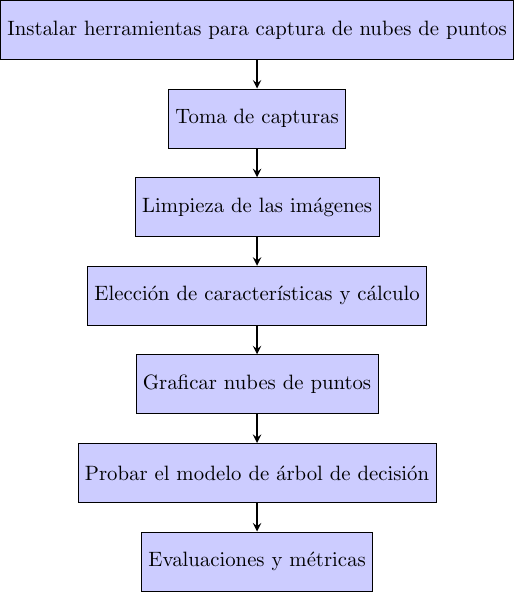
\includegraphics[width=0.5\linewidth]{images/diagrama-1.png}
    \caption{Diagrama representativo del flujo de trabajado }
    \label{fig:diagrama-1}
\end{figure}
\subsection{Toma de fotos}
Para la toma de foto se realizaron diversos experimentos en distintos escenarios. El primero de ellos fue poner un objeto dentro de una caja con material de cuero negro. Sin embargo, se obtenían demasiados puntos del fondo, por lo que se optó por utilizar vasos de vidrio y colocar sobre ellos cada objeto, como se puede observar en la figura \ref{fig:figuraMono}. En detalle la tabla \ref{tab:fotos}, donde muestra las fotos tomadas con color, profundidad y la nube de puntos

\begin{figure}[h]
    \centering
    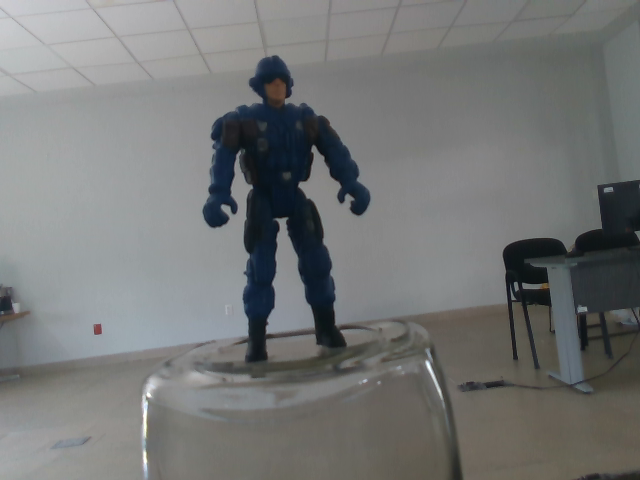
\includegraphics[width=\columnwidth]{prueba_color.png}
    \caption{Muestra de ejemplo de la toma de fotos}
    \label{fig:figuraMono}
\end{figure}


\begin{itemize}
    \item Figura de juguete: 10 cm de alto y 4 cm de largo. La foto se realizo a una distancia de 25 cms y se elevo la cámara 18 cms
    \item Coche: 30 cm de largo y 12 cm de ancho. La foto se realizo a una distancia de 25 cms y se elevo la cámara 18 cms
    \item Cono: 17 cm de largo y 8 cm de ancho. La foto se realizo a una distancia de 25 cms la cámara unicamente contaba con su trípode
    \item Botella de cloro: 39.5 cm de altura y 13.4 cm de largo. La foto se realizo a una distancia de 25 cms y se elevo la cámara 18 cms
    \item Taza: 10 cm de altura y 8 cm de diámetro. La foto se realizo a una distancia de 25 cms y se elevo la cámara 18 cms
    \item Silla: 79 cm de altura, 47 cm de largo y 48 cm de ancho. La foto se tomo a 60 cms de la silla y se elevo la cámara a 40 cms 
\end{itemize}

\subsection{Proceso de filtrado}
Para filtrar las tomas de imágenes, se aplicó la norma L2 o euclidiana, para todos los objetos exceptuando la silla, el rango fue de  $[0,0.25]$, metros y para la silla $[0,1.00]$ De esta manera, se eliminaba una cantidad considerable de fondo, aunque persiste ruido en ciertas tomas. Posteriormente se procede a hacer un análisis exhaustivo en cada imagen, recortando regiones innecesarias. 
\begin{table}[h]
  \centering
  \caption{Tabla 7x4 con descripciones y ejemplos de imágenes}
  \label{tab:fotos}
  \setlength{\tabcolsep}{4pt}
  \renewcommand{\arraystretch}{1.05}
  \begin{tabular}{|>{\centering\arraybackslash}m{0.18\columnwidth}|
                  >{\centering\arraybackslash}m{0.23\columnwidth}|
                  >{\centering\arraybackslash}m{0.23\columnwidth}|
                  >{\centering\arraybackslash}m{0.23\columnwidth}|}
    \hline
    \textbf{Objeto} & \textbf{Imagen a color} & \textbf{Imagen de profundidad} & \textbf{Nube de puntos} \\
    \hline
    Cloro &
    \adjustbox{max width=\linewidth,max height=2cm}{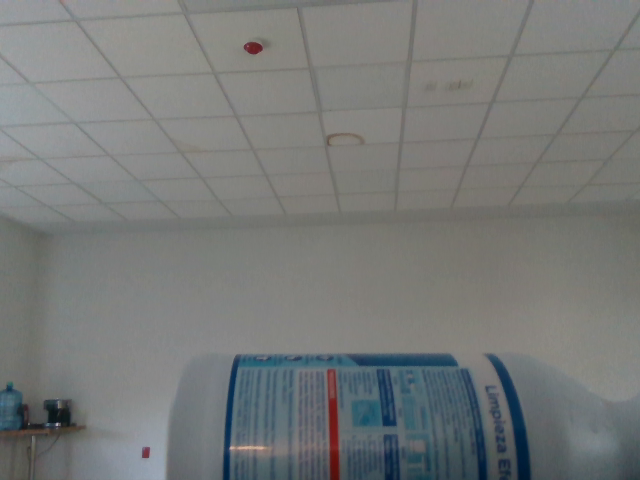
\includegraphics{images/cloro_imagen_prof/prueba_color.png}} &
    \adjustbox{max width=\linewidth,max height=2cm}{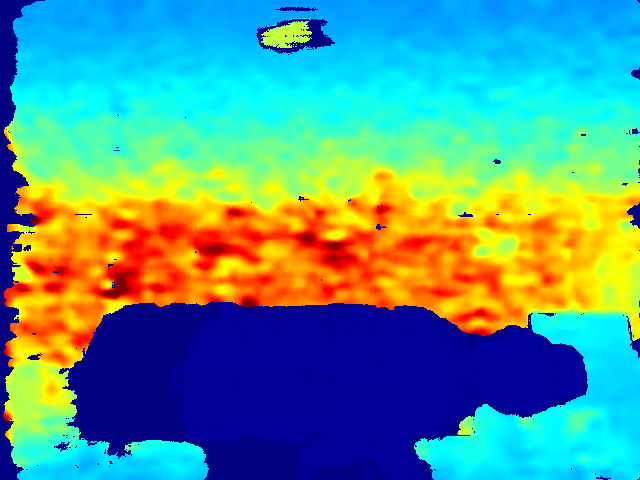
\includegraphics{images/cloro_imagen_prof/prueba_profundidad.png}} &
    \adjustbox{max width=\linewidth,max height=2cm}{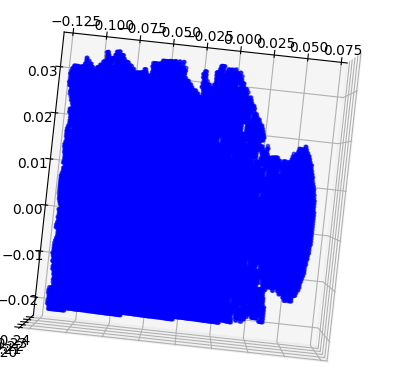
\includegraphics{images/cloro_imagen_prof/image.png}} \\
    \hline
    Coche &
    \adjustbox{max width=\linewidth,max height=2cm}{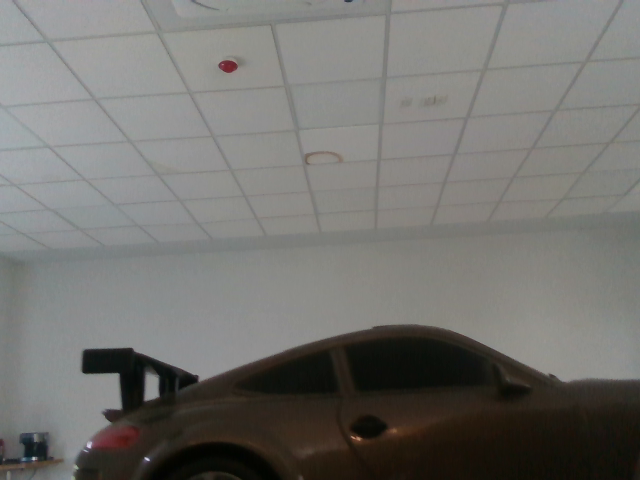
\includegraphics{images/coche_color_prof/prueba_color.png}} &
    \adjustbox{max width=\linewidth,max height=2cm}{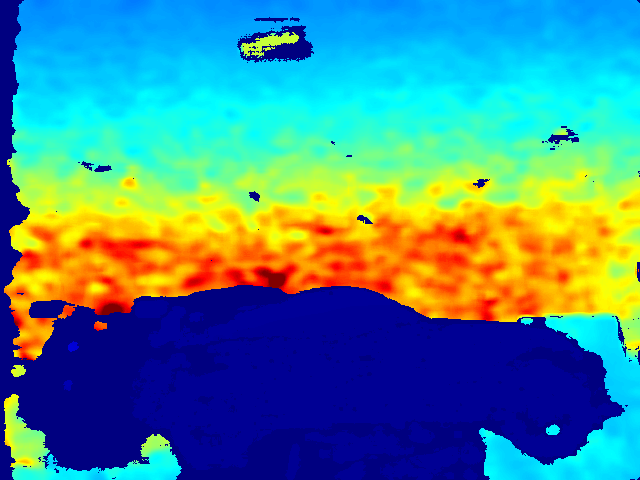
\includegraphics{images/coche_color_prof/prueba_profundidad.png}} &
    \adjustbox{max width=\linewidth,max height=2cm}{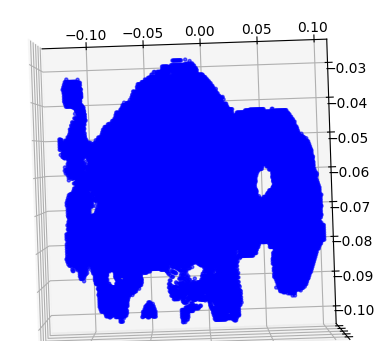
\includegraphics{images/coche_color_prof/image.png}} \\
    \hline
    Cono &
    \adjustbox{max width=\linewidth,max height=2cm}{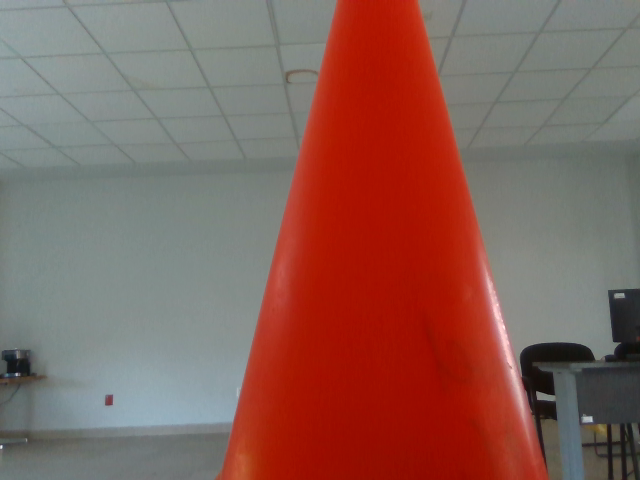
\includegraphics{images/cono_imagen_prof/prueba_color.png}} &
    \adjustbox{max width=\linewidth,max height=2cm}{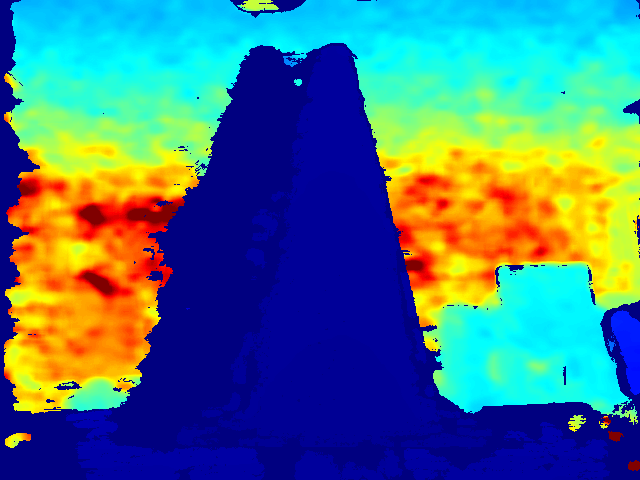
\includegraphics{images/cono_imagen_prof/prueba_profundidad.png}} &
    \adjustbox{max width=\linewidth,max height=2cm}{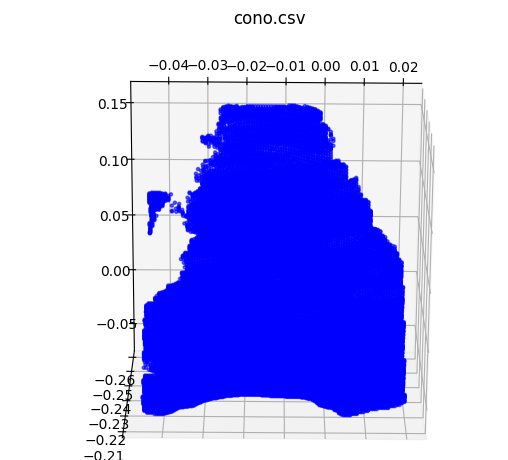
\includegraphics{images/cono_imagen_prof/image.png}} \\
    \hline
    Monito &
    \adjustbox{max width=\linewidth,max height=2cm}{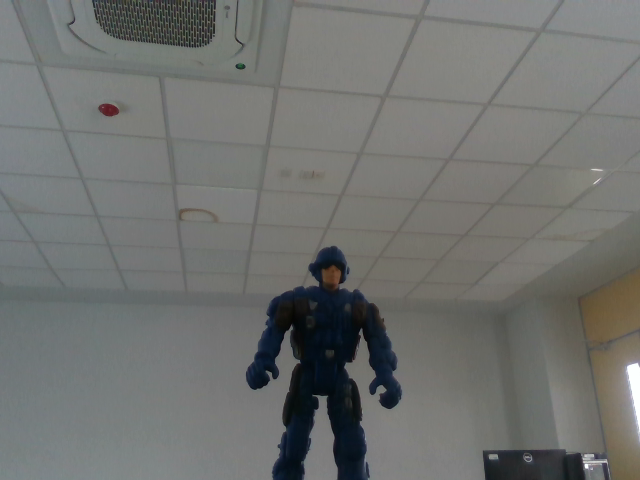
\includegraphics{images/monito_col_prof/prueba_color.png}} &
    \adjustbox{max width=\linewidth,max height=2cm}{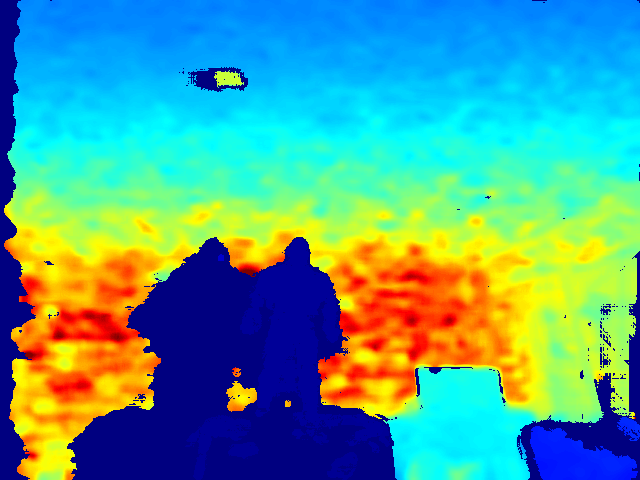
\includegraphics{images/monito_col_prof/prueba_profundidad.png}} &
    \adjustbox{max width=\linewidth,max height=2cm}{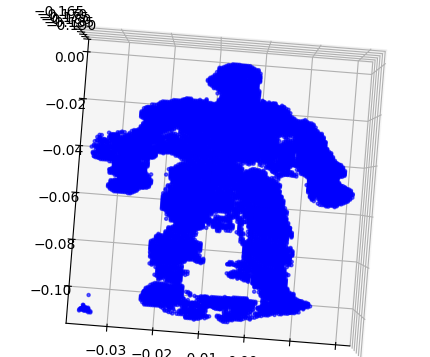
\includegraphics{images/monito_col_prof/image.png}} \\
    \hline
    Silla &
    \adjustbox{max width=\linewidth,max height=2cm}{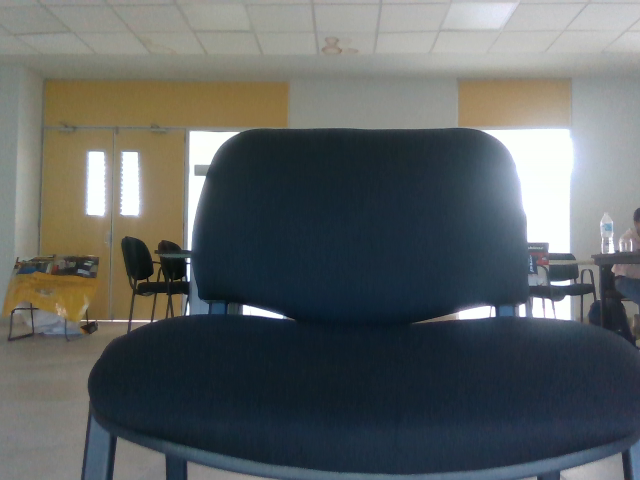
\includegraphics{images/silla_prof_col/prueba_color.png}} &
    \adjustbox{max width=\linewidth,max height=2cm}{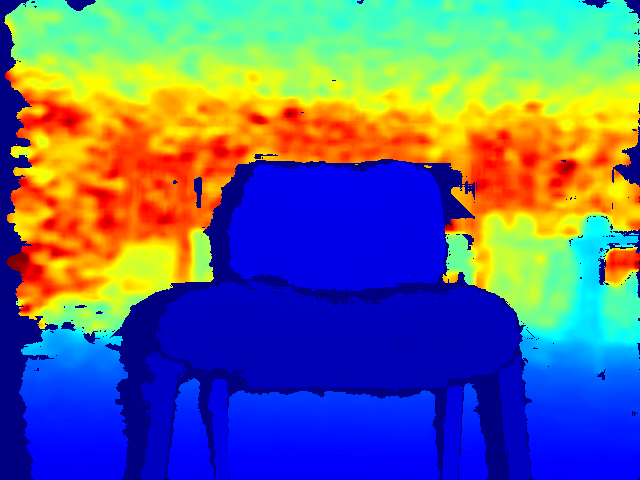
\includegraphics{images/silla_prof_col/prueba_profundidad.png}} &
    \adjustbox{max width=\linewidth,max height=2cm}{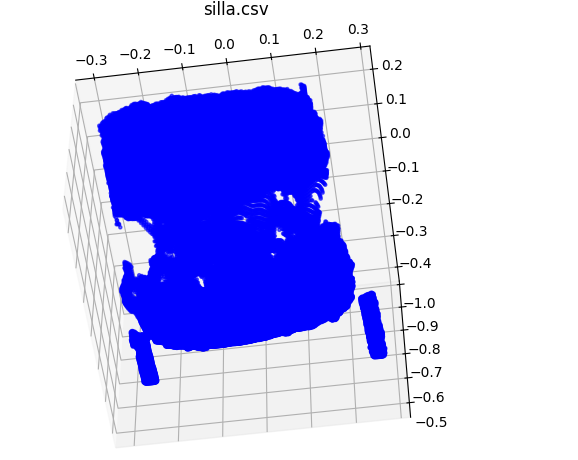
\includegraphics{images/silla_prof_col/image.png}} \\
    \hline
    Taza &
    \adjustbox{max width=\linewidth,max height=2cm}{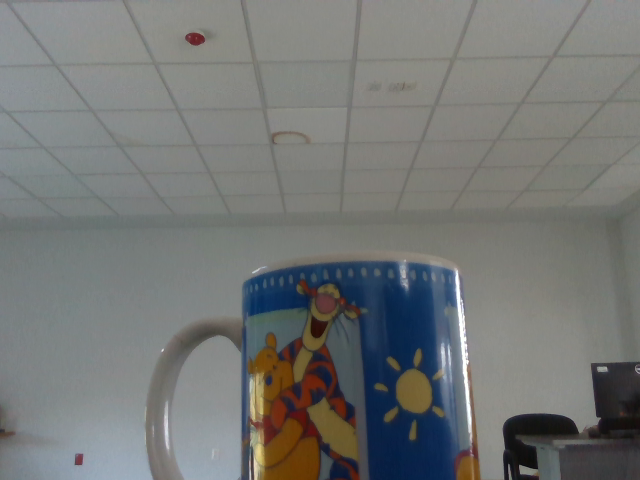
\includegraphics{images/taza_prof_col/prueba_color.png}} &
    \adjustbox{max width=\linewidth,max height=2cm}{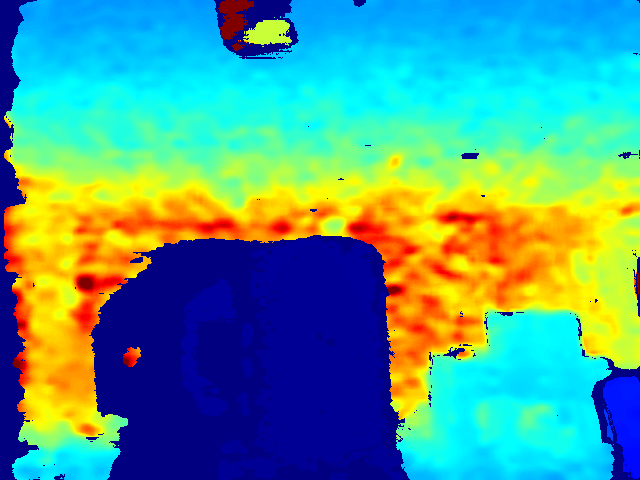
\includegraphics{images/taza_prof_col/prueba_profundidad.png}} &
    \adjustbox{max width=\linewidth,max height=2cm}{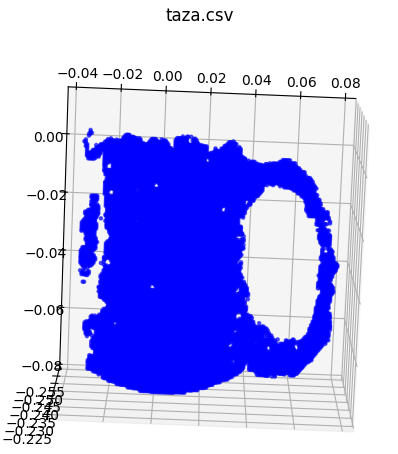
\includegraphics{images/taza_prof_col/image.png}} \\
    \hline
  \end{tabular}
\end{table}
\subsection{calculo de las características}
Se calcularon 10 características, sin embargo, es una cantidad muy reducidad, por lo que en base a una imagen se submuestra aleatoriamente al 20\%,30\%,40\% y 50 \%
 características nuevas. La lista de características calculadas es la siguiente:

 \begin{itemize}
     \item Volumen
     \item dimensión x
     \item dimensión y
     \item dimensión z
      \item Centroide x
     \item Centroide y
     \item Centroide z
     \item curvatura 
      \item borde
     \item FPFH
 \end{itemize}
 Sin embargo, se sabe bien que el volumen y la dimensión solo son características redundantes, por lo tanto, se pueden omitir, ya sea el volumen y la dimensión, sin embargo, de manera ilustrativa, podemos ver y calcular su correlación para poder decir que ambos poseen alta relación,(aunque con el simple hecho de que el volumen corresponde a las distancias x,y,z), por lo tanto, se puede eliminar el volumen y en su lugar, calcular la compacidad.
 \subsubsection{Compacidad}
 Consiste en el siguiente cálculo
 $\frac{volumen}{d_x\cdot d_y\cdot d_z}$
 Indica lo compactado que puede estar un objeto. EL volumen es resultado de un ConvexHull, este cálculo viene dentro del paquete scipy.spatial

 \subsubsection{Dimensiones}
 Consisten únicamente en la longitud del punto más alejado y más cercano de cada eje
 \subsection{Centroide}
 ES el punto central de cada eje se calcula como
 $$\frac{1}{n}\sum^n_{i=0} x_i$$
 \subsubsection{Curvatura}
 $$C=Cov(\{p_i\}) \in \mathbb{R}^{3\times 3}$$ Siendo esta la curvatura, se hace el cálculo de sus autovalores
 $$k(p)=\frac{\lambda_0}{\lambda_0+\lambda_1+\lambda_2}$$
 Finalmente se calcula su media $Curvatura=\frac{1}{N}\sum_{p}k(p)$ sobre todos los puntos
 En si, tiene que hacer el calculo de los k vecinos de puntos, por lo que tiene internamente un knn. El cálculo se realiza con el uso del paquete open3d y numpy.
 \subsubsection{Feature border}:
 En este se calcula el convex hull del volumen y se divide por la cantidad $N$ de puntos. Se utiliza la librería de scipy.spatial
 \subsection{FPFH}
 Primeramente se calculan sus frecuencias, sin embargom lo hace por bloques dentro del conjunto, se realiza una media de frecuencias, sucesviamente se normaliza y finalmente se calcula su entropía.
 $$\bar{f}=\frac{1}{N}\sum^N_{i=1}f_i \in \mathbb{R}^d$$
 $$p_j=\frac{\bar{f}_j}{\sum^d_{i=1}\bar{f}_i}$$
 $$H(p)=-\sum^d_{i=1}p_i\log(p_i+\epsilon)$$
 De esta manera con el $\epsilon$ se evita tener valores de 0. Todos estos calculos se ralizan con open 3d y numpy.
 Por medio de las siguientes gráficas de la tabla \ref{tab:caracteristicas_grupos_1} y la tabla \ref{tab:caracteristicas_grupos_2}, podemos visualizar este comportamiento, en el que ninguno de las tres variables posee una relación de correlación.
% Primera mitad
\begin{table}[h]
    \centering
    \caption{Características calculadas por grupo de variables (Parte 1)}
    \label{tab:caracteristicas_grupos_1}
    \setlength{\tabcolsep}{4pt}
    \renewcommand{\arraystretch}{1.2}
    \begin{tabular}{|>{\centering\arraybackslash}m{0.48\columnwidth}|
                    >{\centering\arraybackslash}m{0.48\columnwidth}|}
        \hline
        \textbf{Variables} & \textbf{Ejemplo de visualización} \\
        \hline
        dx\_frac20, dy\_frac20, dz\_frac20 & 
        \adjustbox{max width=\linewidth,max height=3cm}{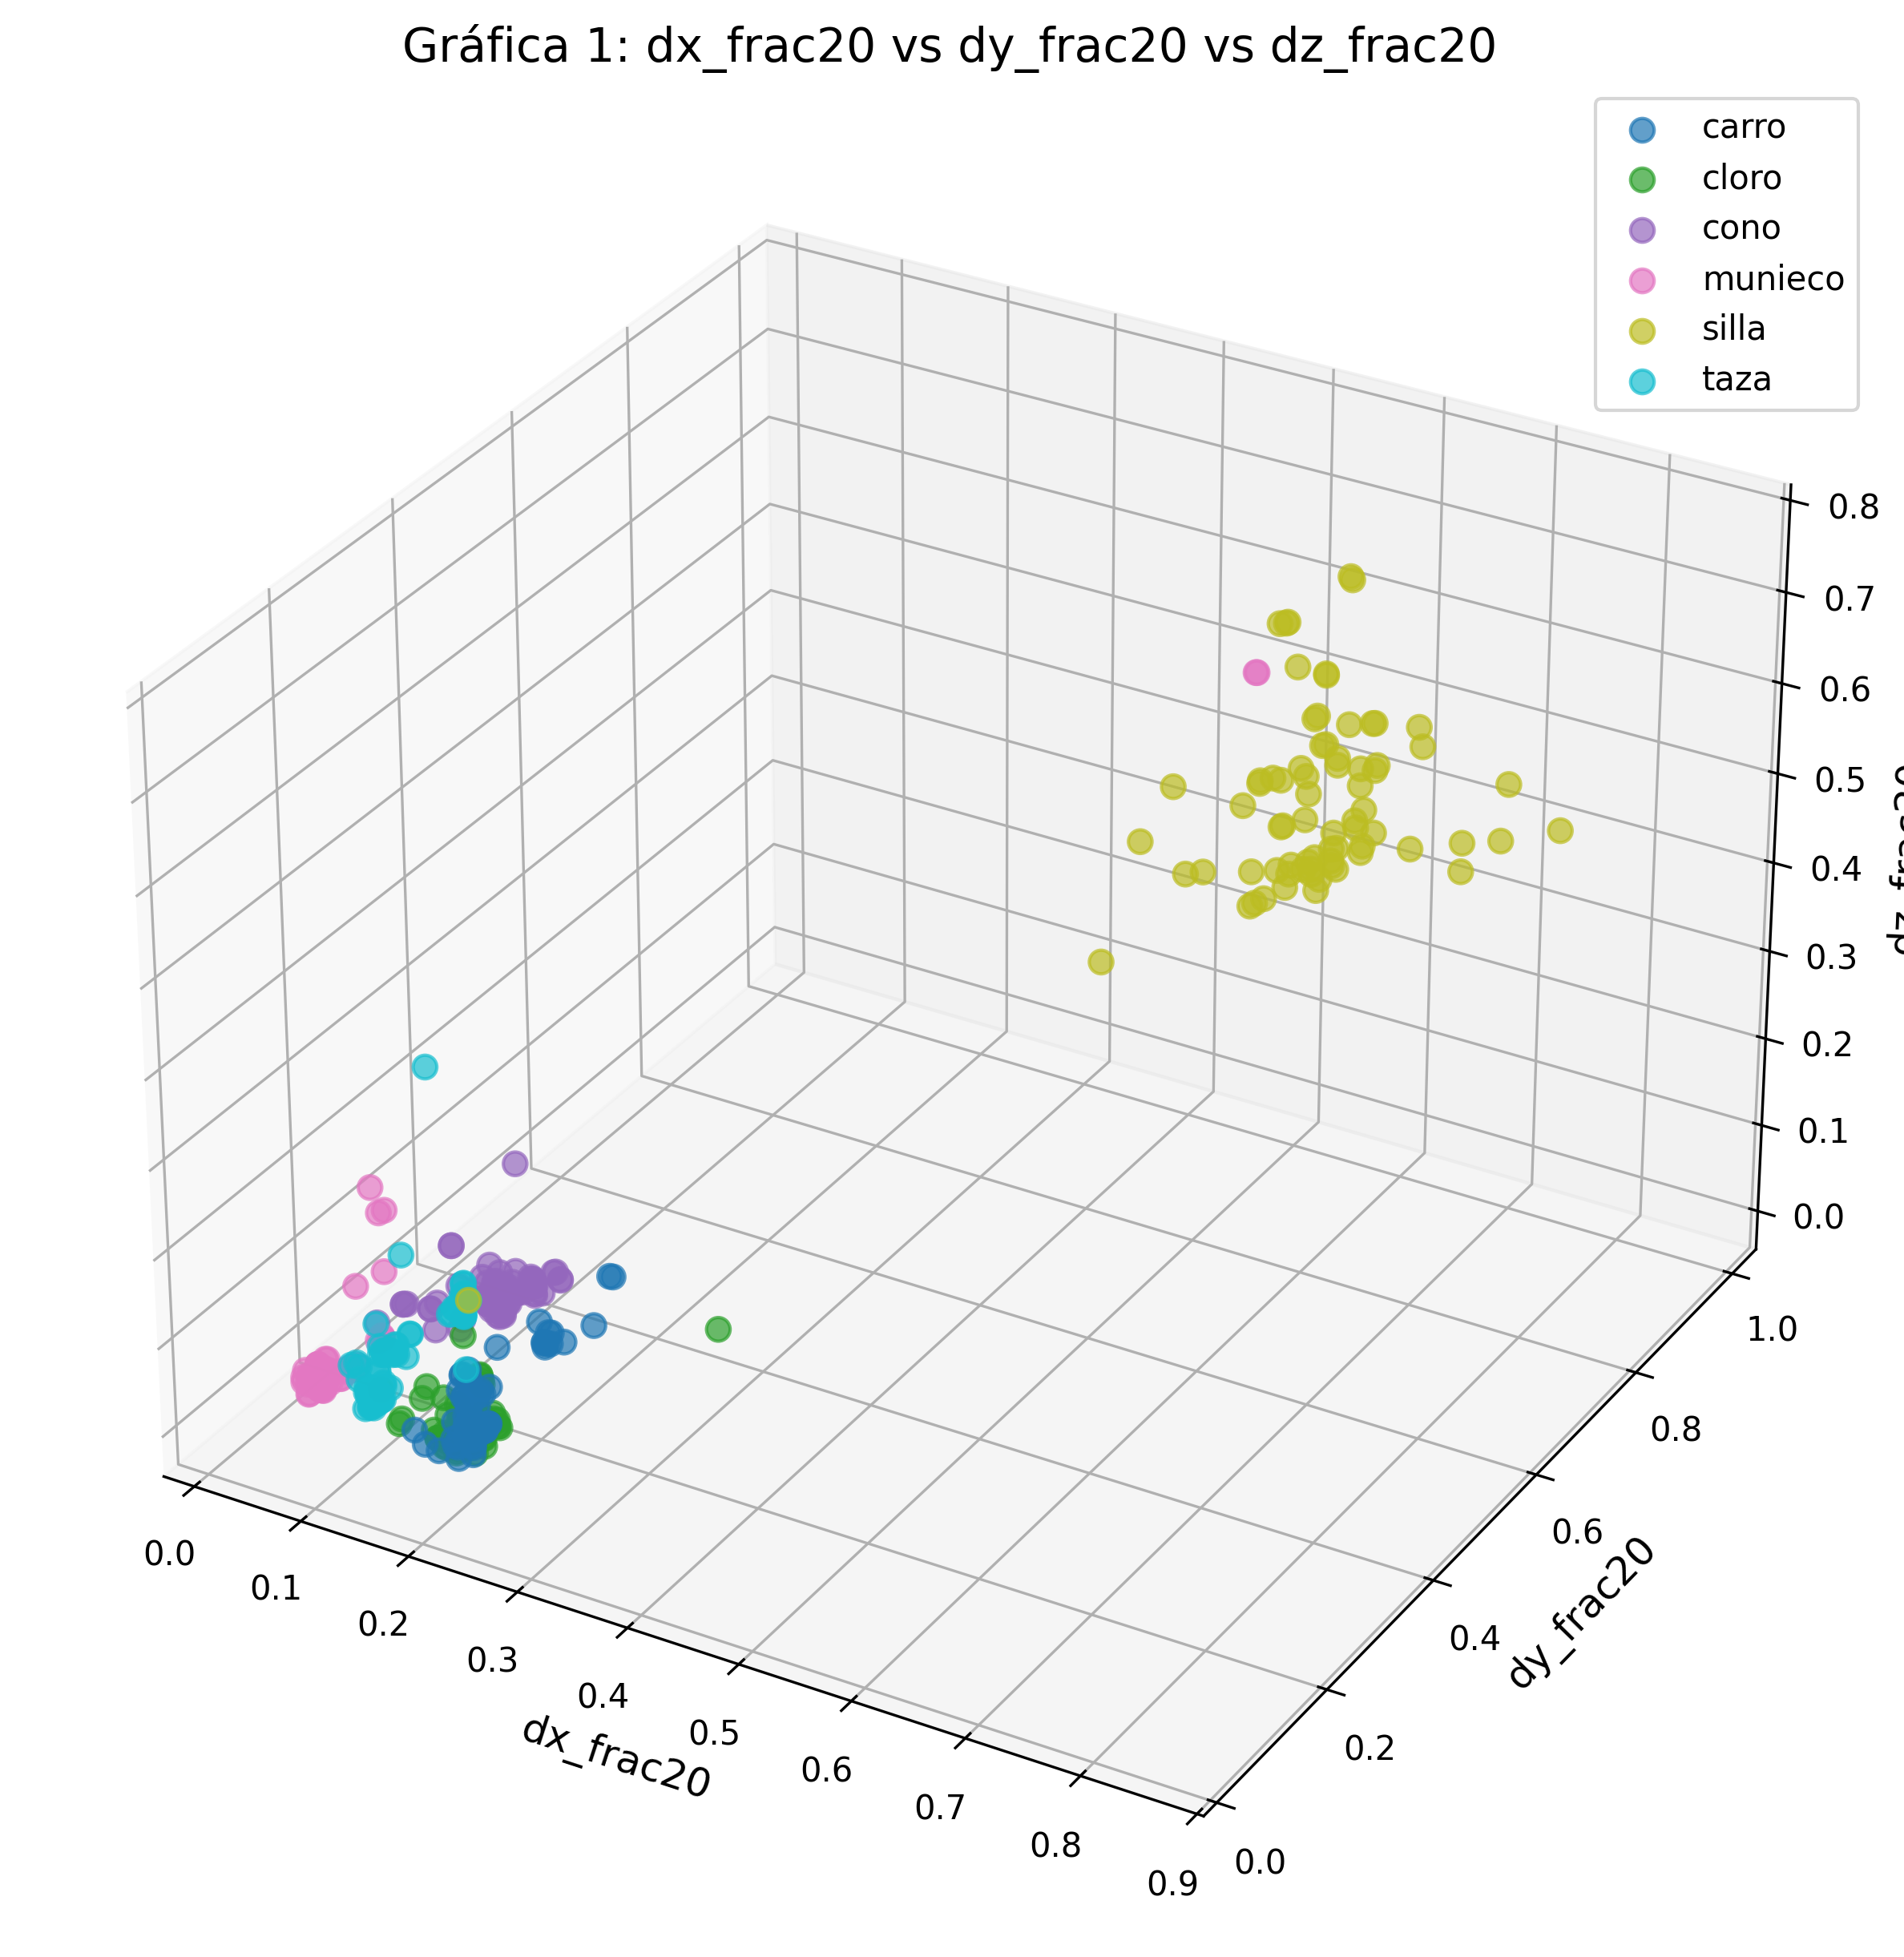
\includegraphics{images/variables/grafica_combinada_01.png}} \\
        \hline
        cx\_frac20, cy\_frac20, cz\_frac20 & 
        \adjustbox{max width=\linewidth,max height=3cm}{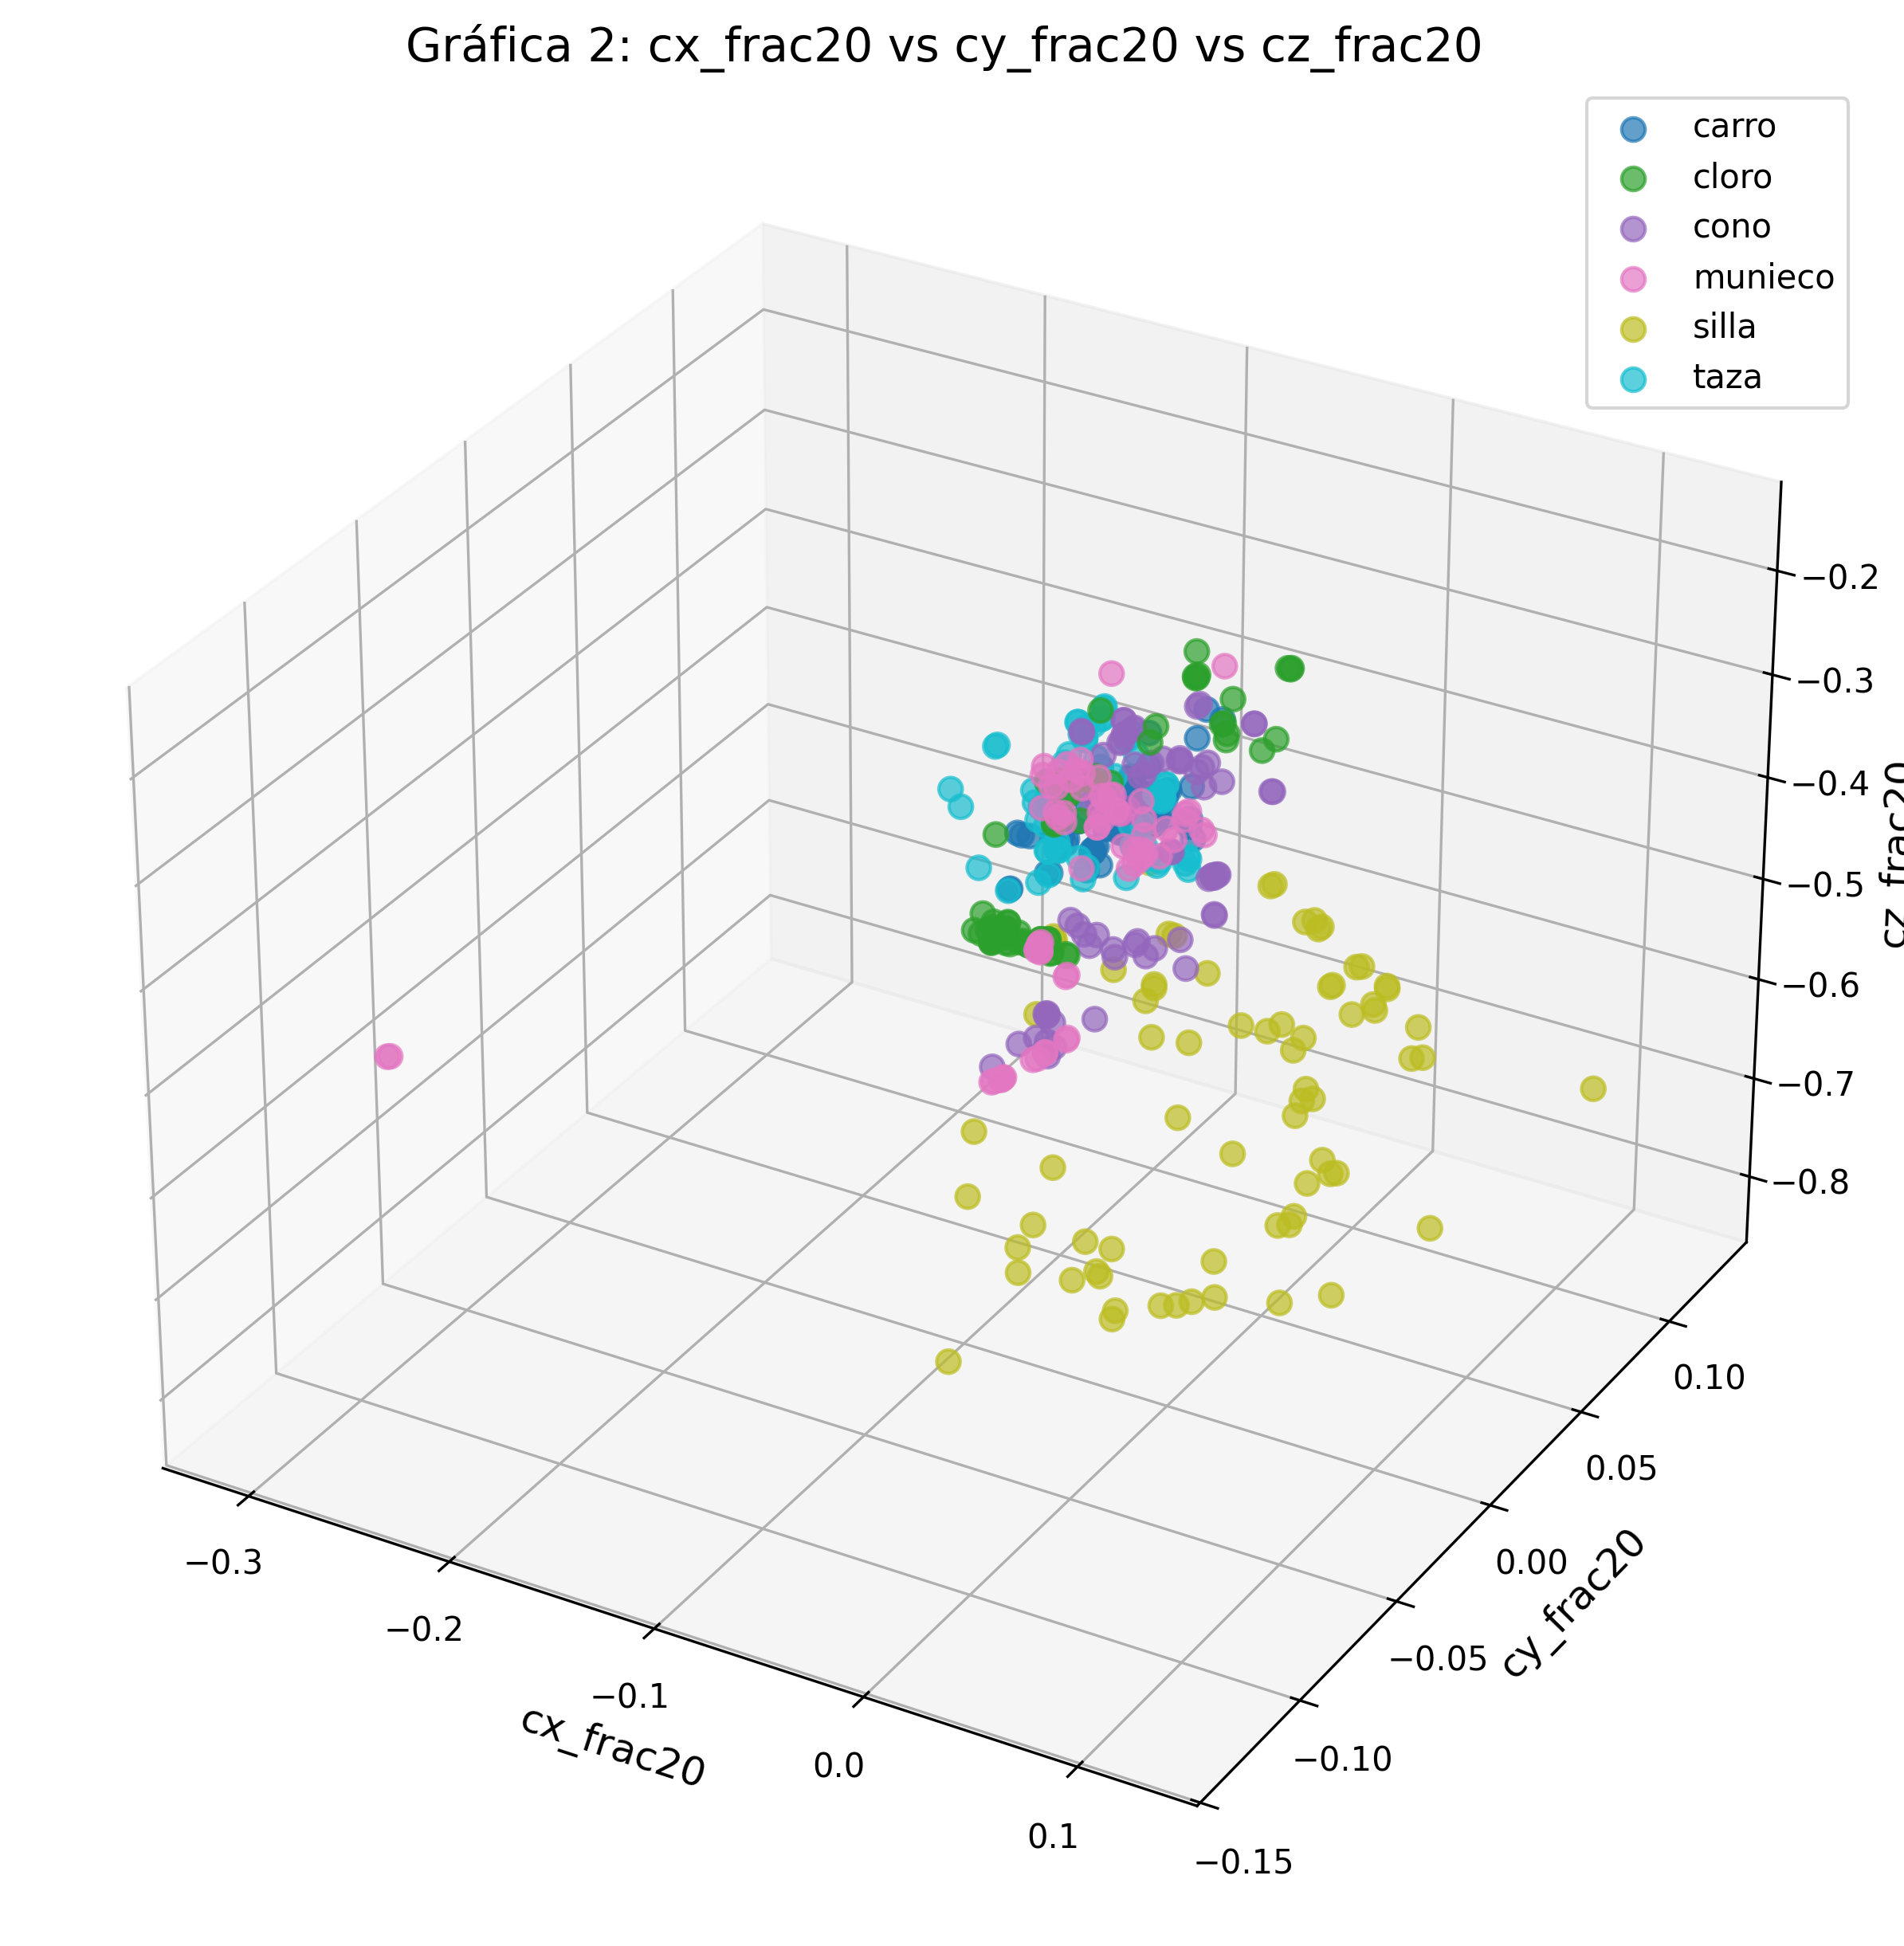
\includegraphics{images/variables/grafica_combinada_02.png}} \\
        \hline
        curvature\_frac20, border\_frac20, compacidad\_frac20 & 
        \adjustbox{max width=\linewidth,max height=3cm}{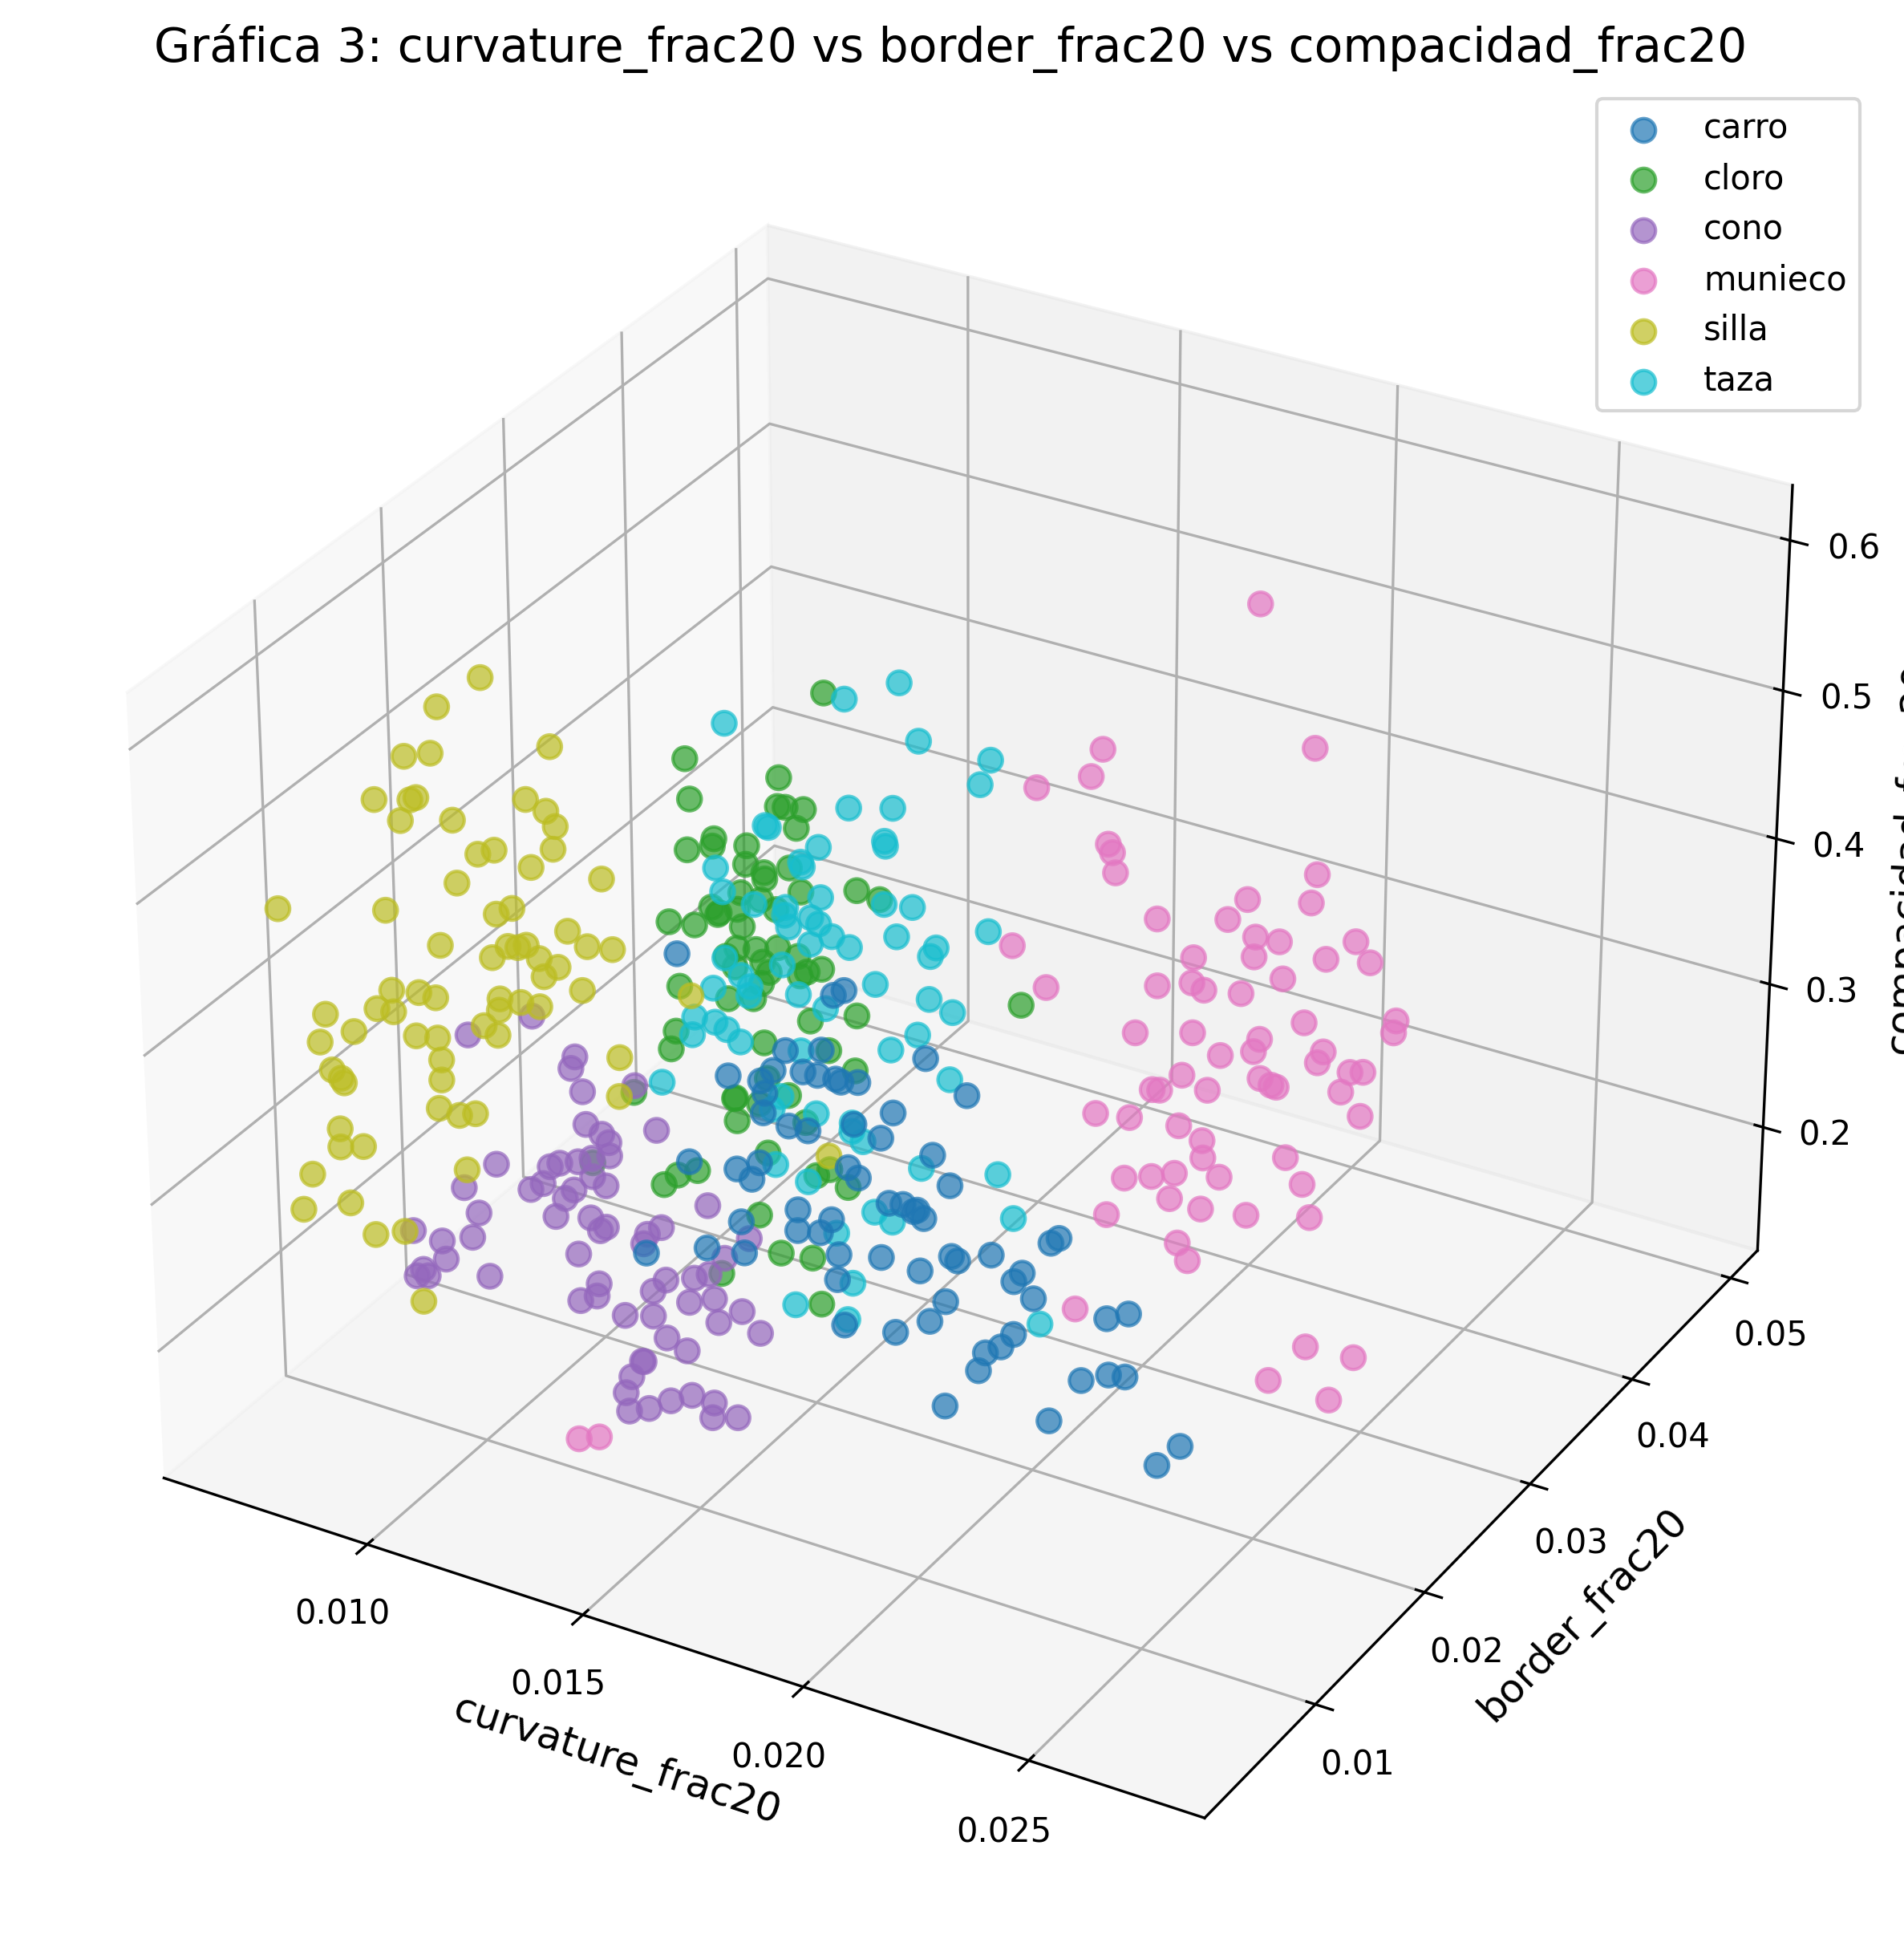
\includegraphics{images/variables/grafica_combinada_03.png}} \\
        \hline
        fpfh\_frac20, dx\_frac30, dy\_frac30 & 
        \adjustbox{max width=\linewidth,max height=3cm}{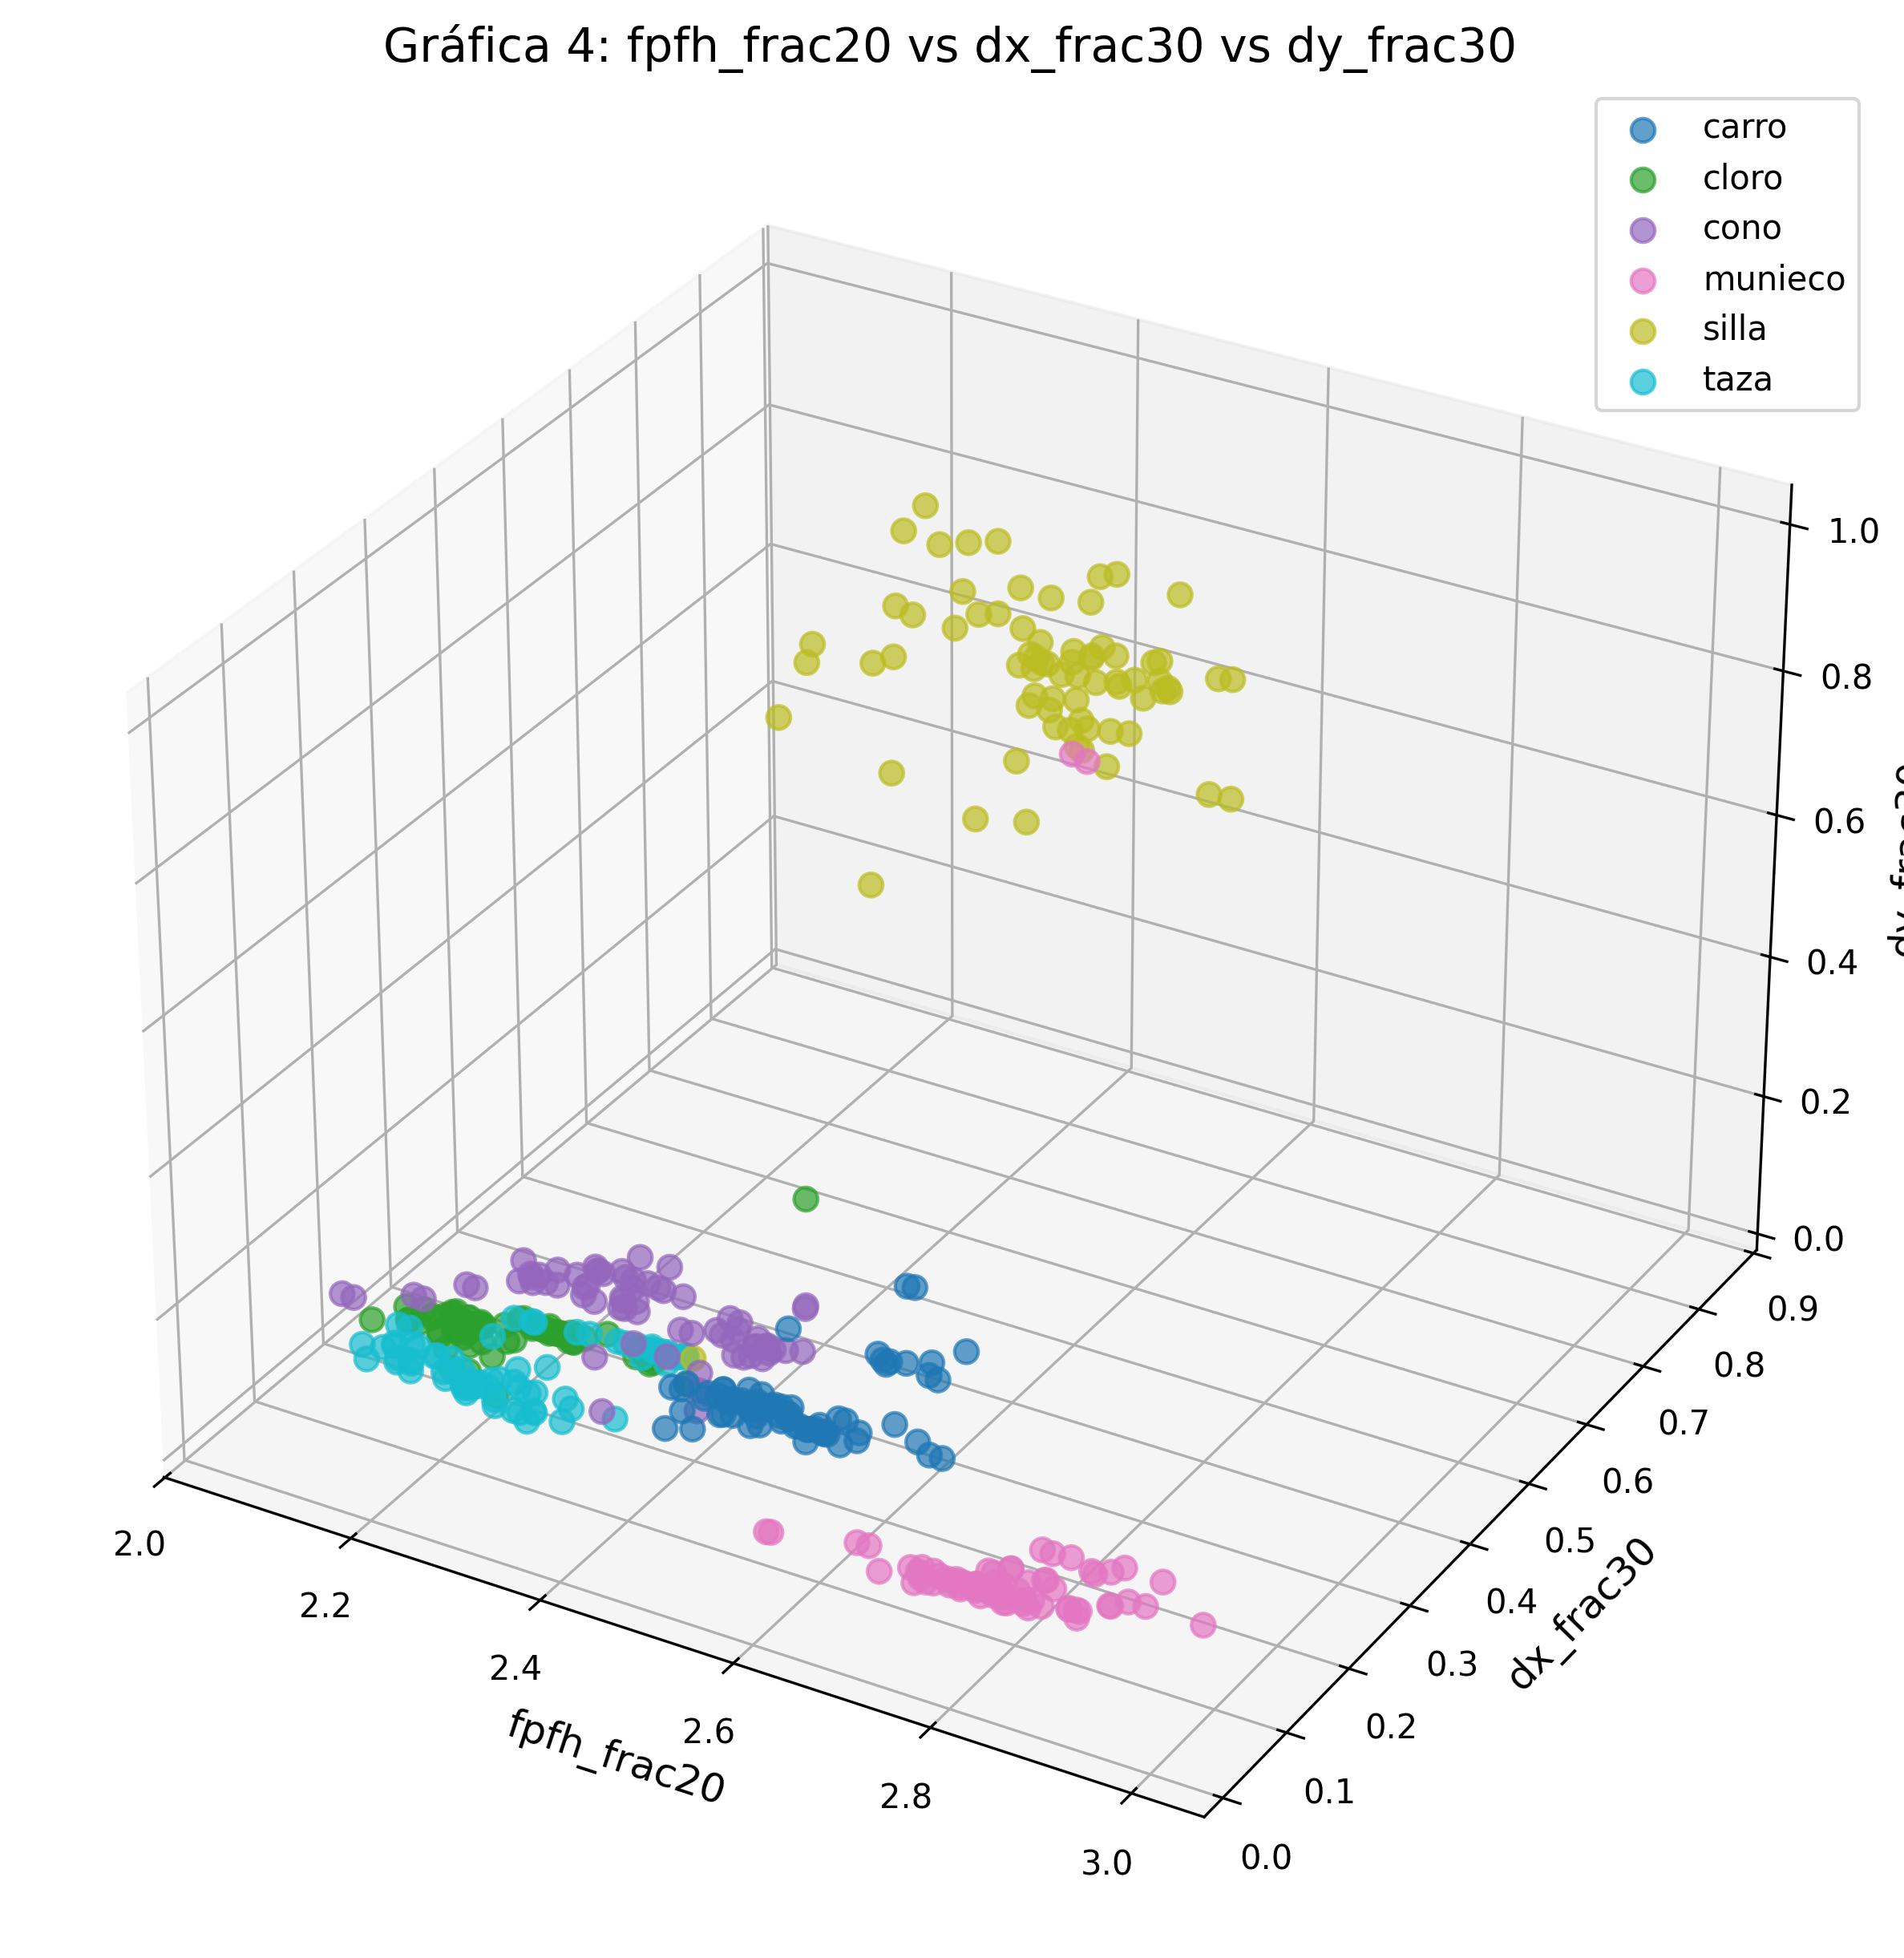
\includegraphics{images/variables/grafica_combinada_04.png}} \\
        \hline
        dz\_frac30, cx\_frac30, cy\_frac30 & 
        \adjustbox{max width=\linewidth,max height=3cm}{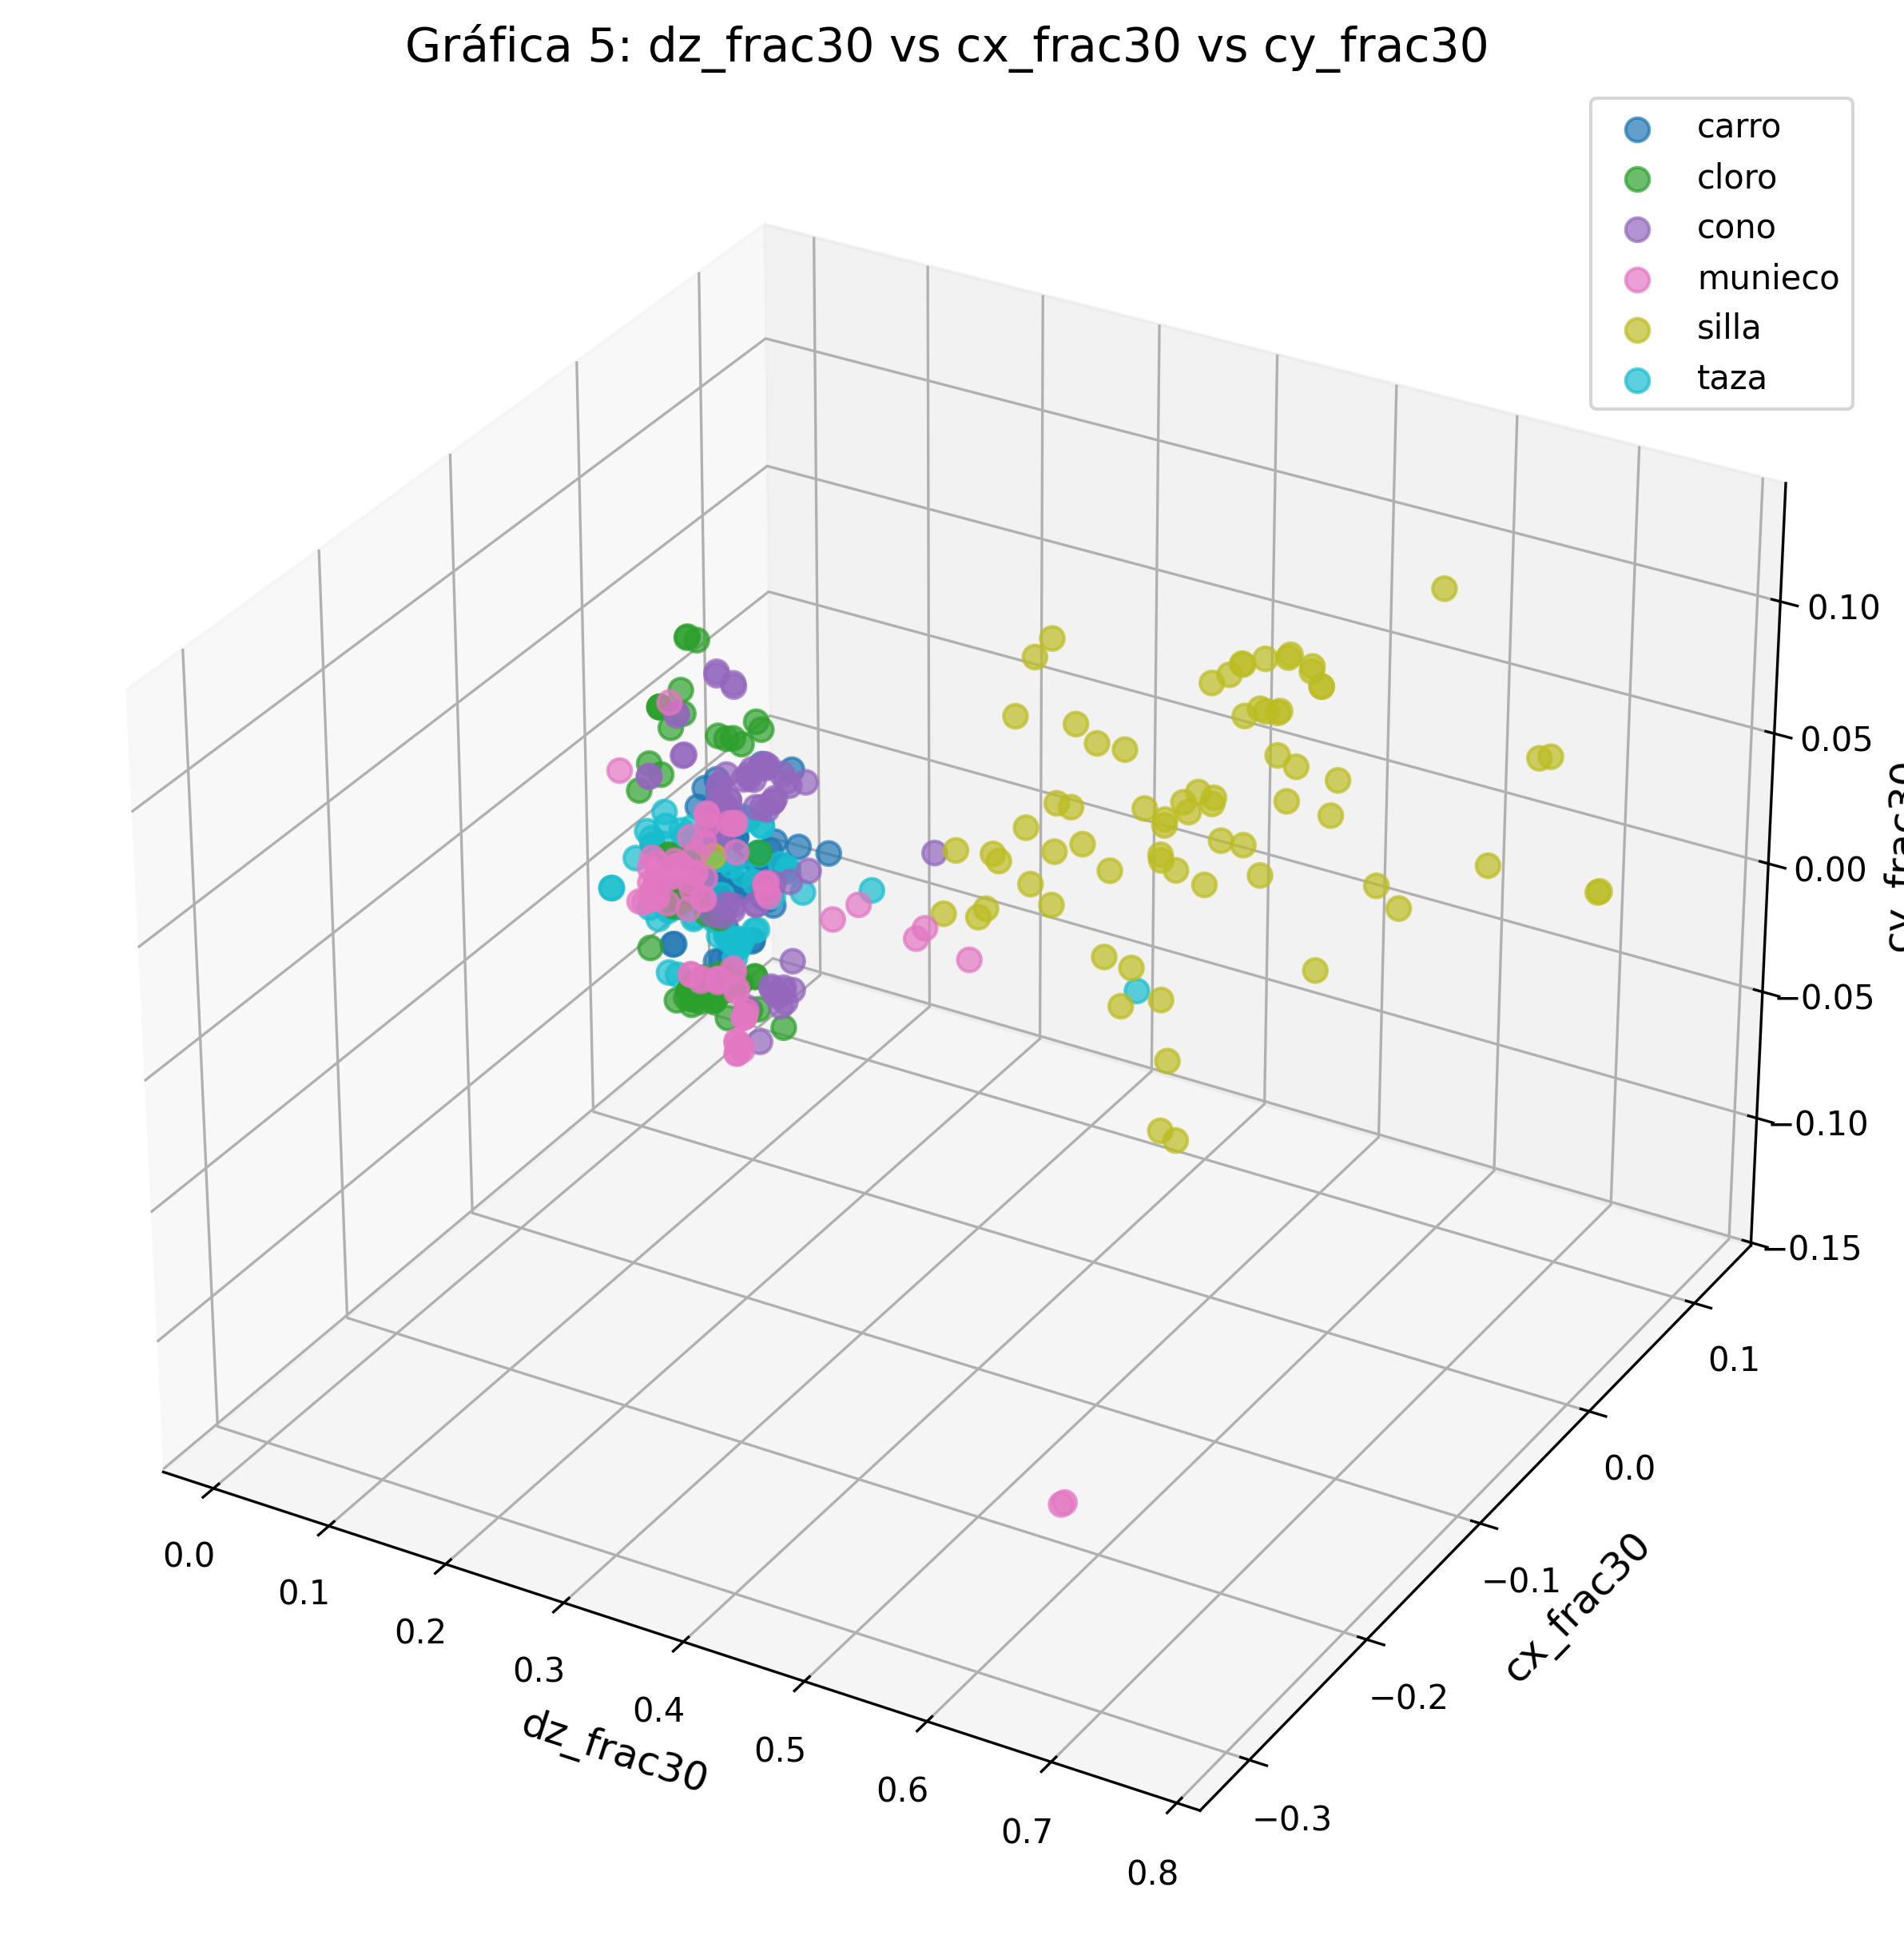
\includegraphics{images/variables/grafica_combinada_05.png}} \\
        \hline
        cz\_frac30, curvature\_frac30, border\_frac30 & 
        \adjustbox{max width=\linewidth,max height=3cm}{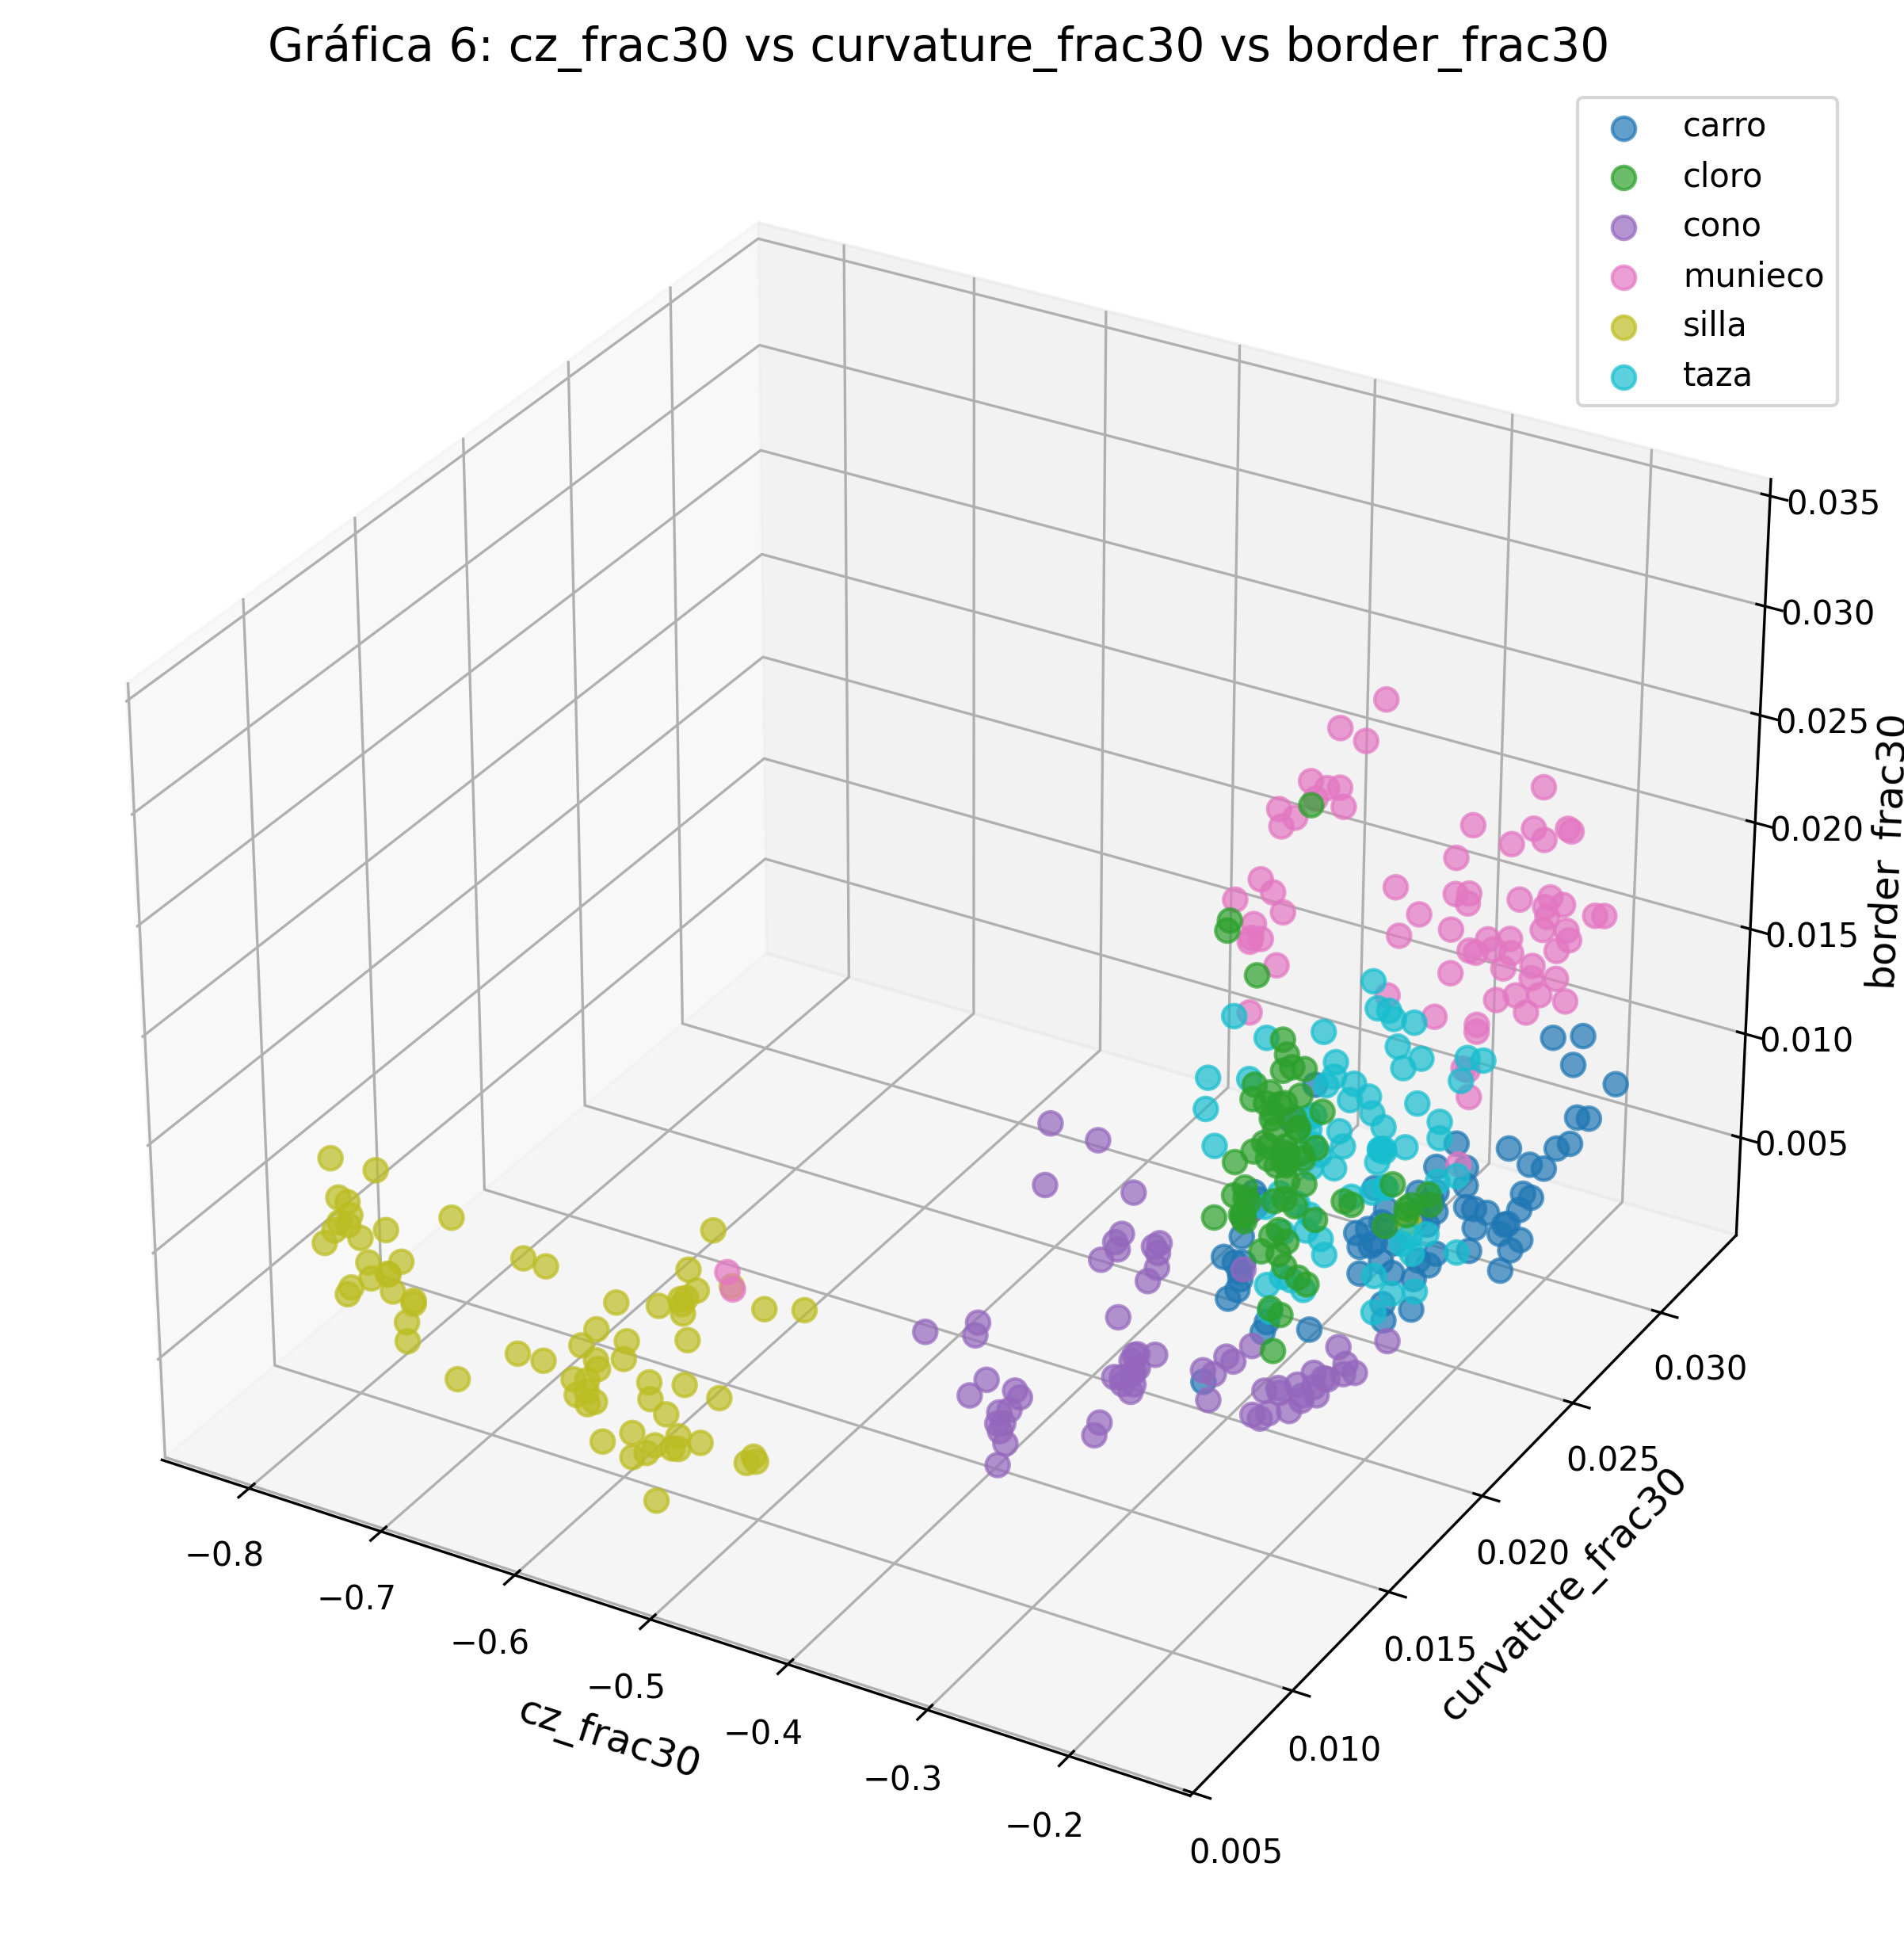
\includegraphics{images/variables/grafica_combinada_06.png}} \\
        \hline
    \end{tabular}
\end{table}

% Segunda mitad
\begin{table}[h]
    \centering
    \caption{Características calculadas por grupo de variables (Parte 2)}
    \label{tab:caracteristicas_grupos_2}
    \setlength{\tabcolsep}{4pt}
    \renewcommand{\arraystretch}{1.2}
    \begin{tabular}{|>{\centering\arraybackslash}m{0.48\columnwidth}|
                    >{\centering\arraybackslash}m{0.48\columnwidth}|}
        \hline
        \textbf{Variables} & \textbf{Ejemplo de visualización} \\
        \hline
        compacidad\_frac30, fpfh\_frac30, dx\_frac40 & 
        \adjustbox{max width=\linewidth,max height=3cm}{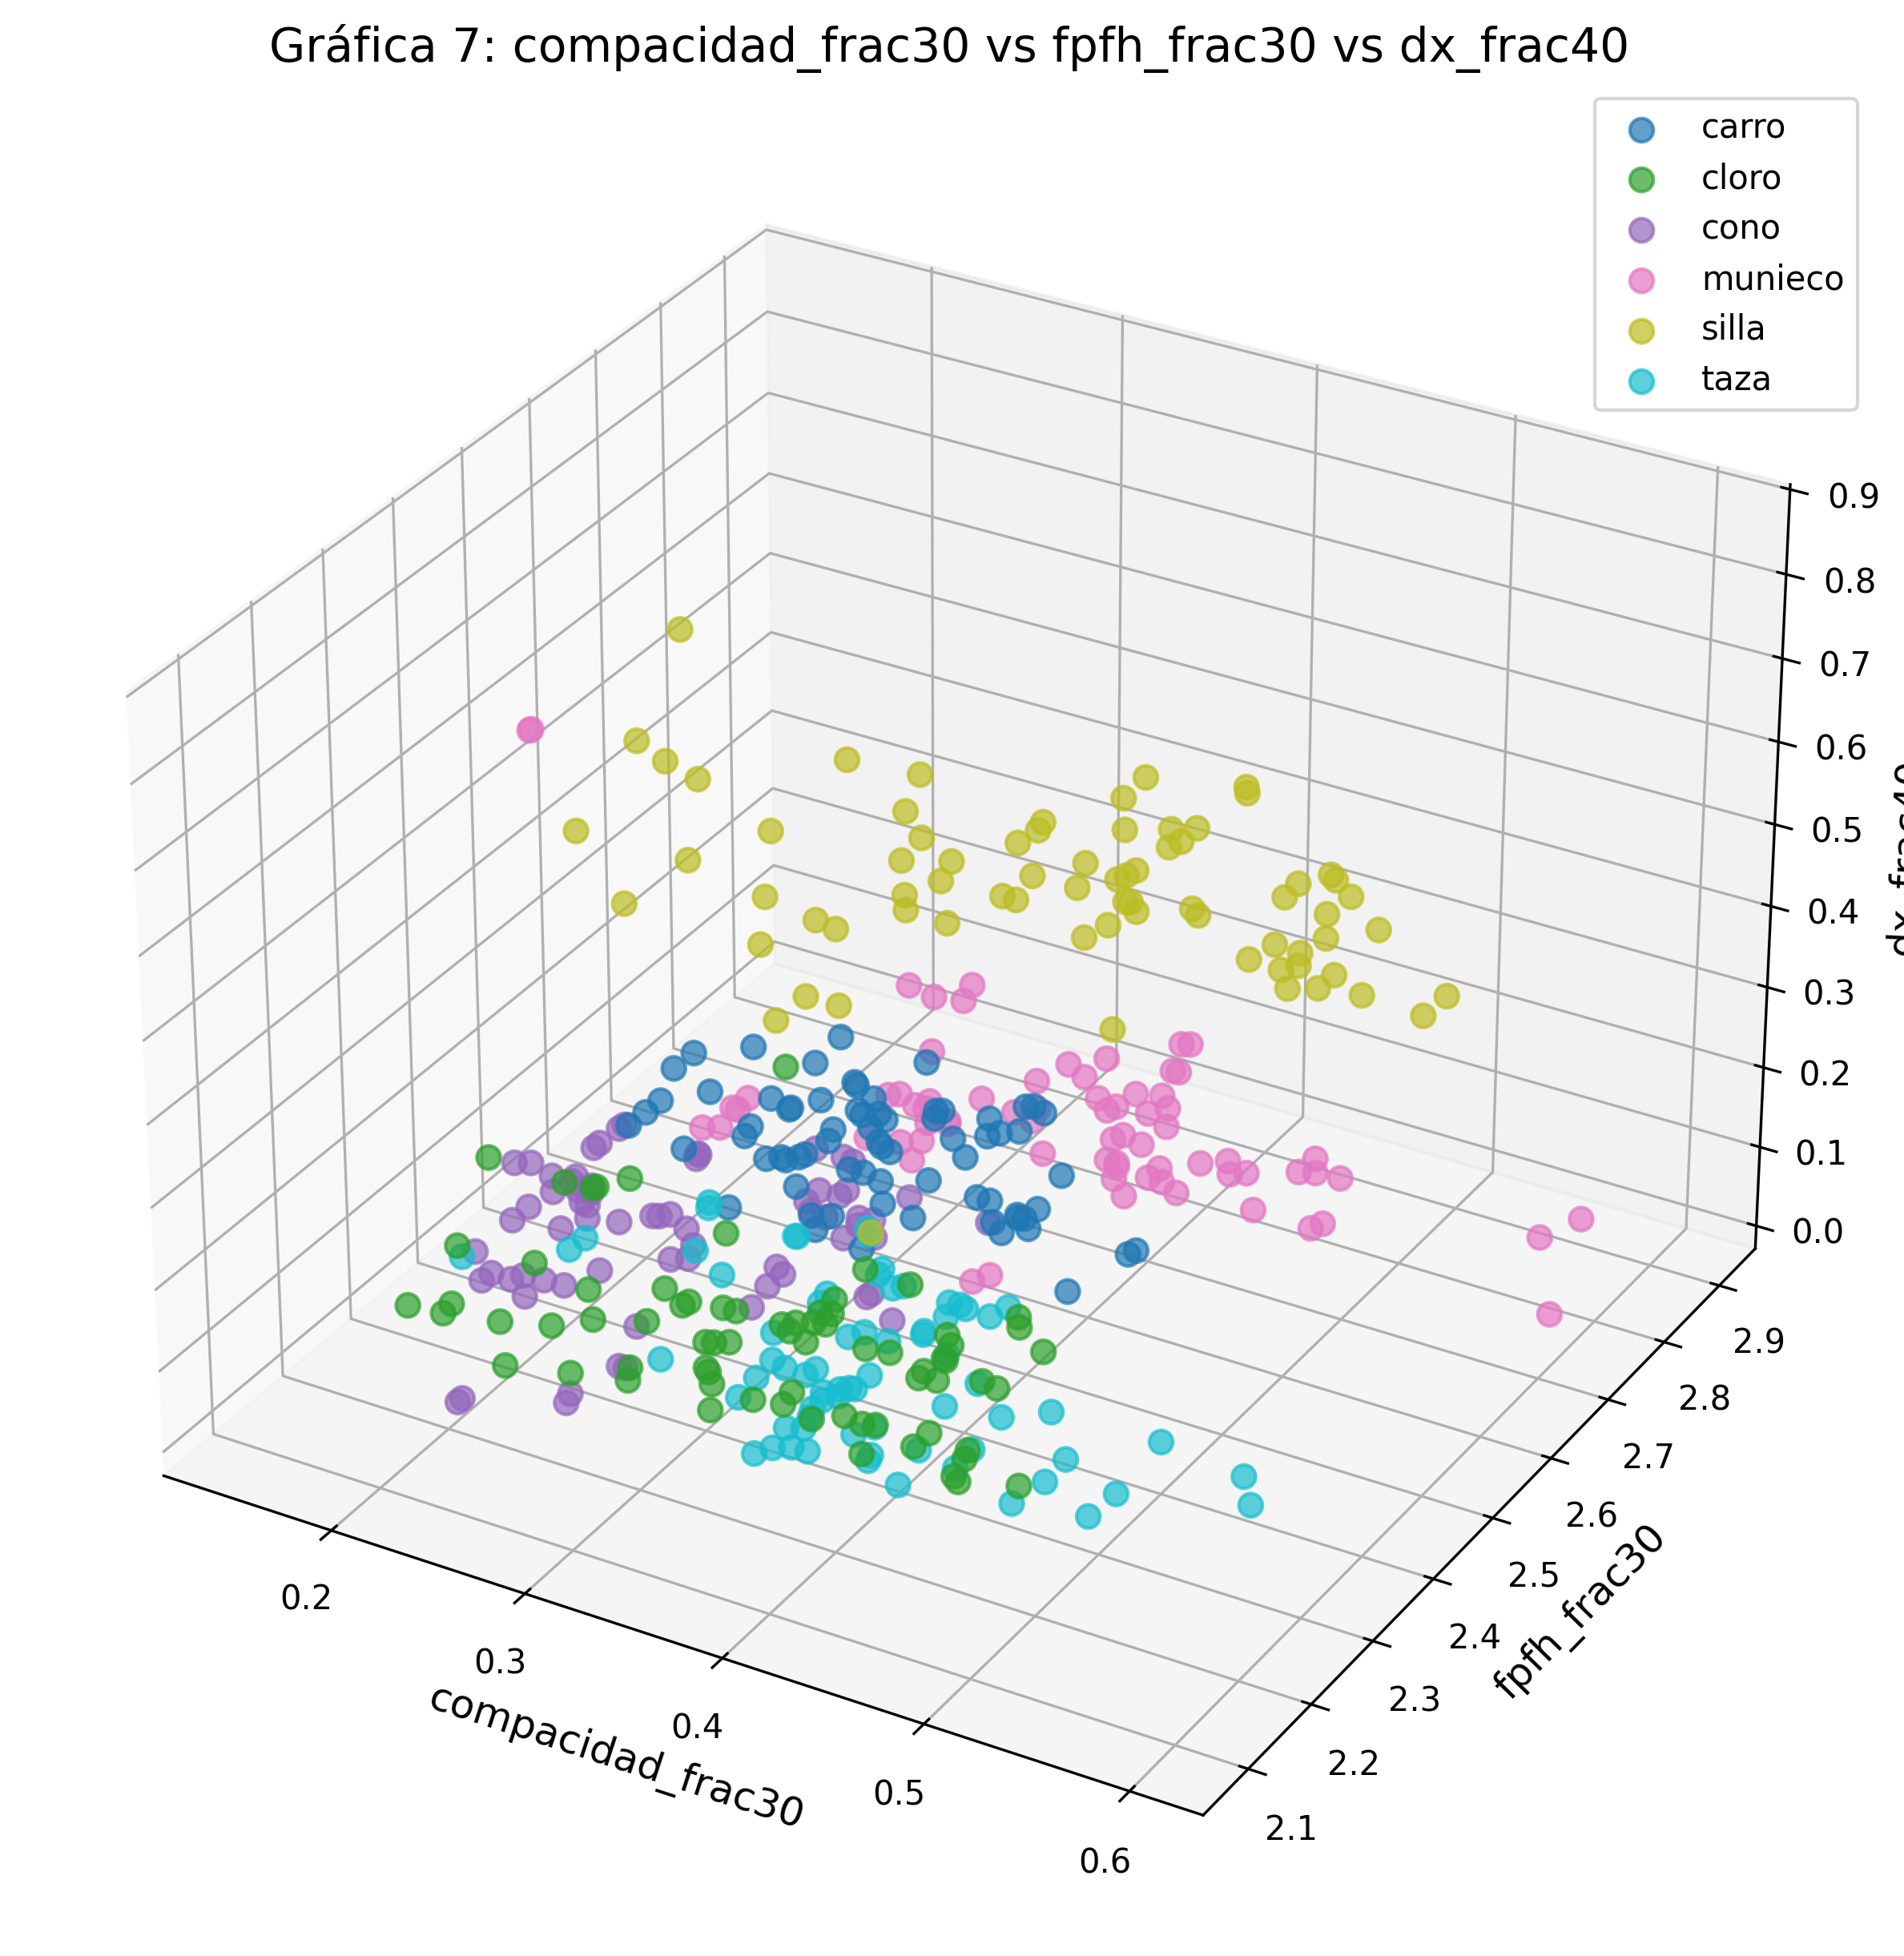
\includegraphics{images/variables/grafica_combinada_07.png}} \\
        \hline
        dy\_frac40,dz\_frac40,cx\_frac40 & 
        \adjustbox{max width=\linewidth,max height=3cm}{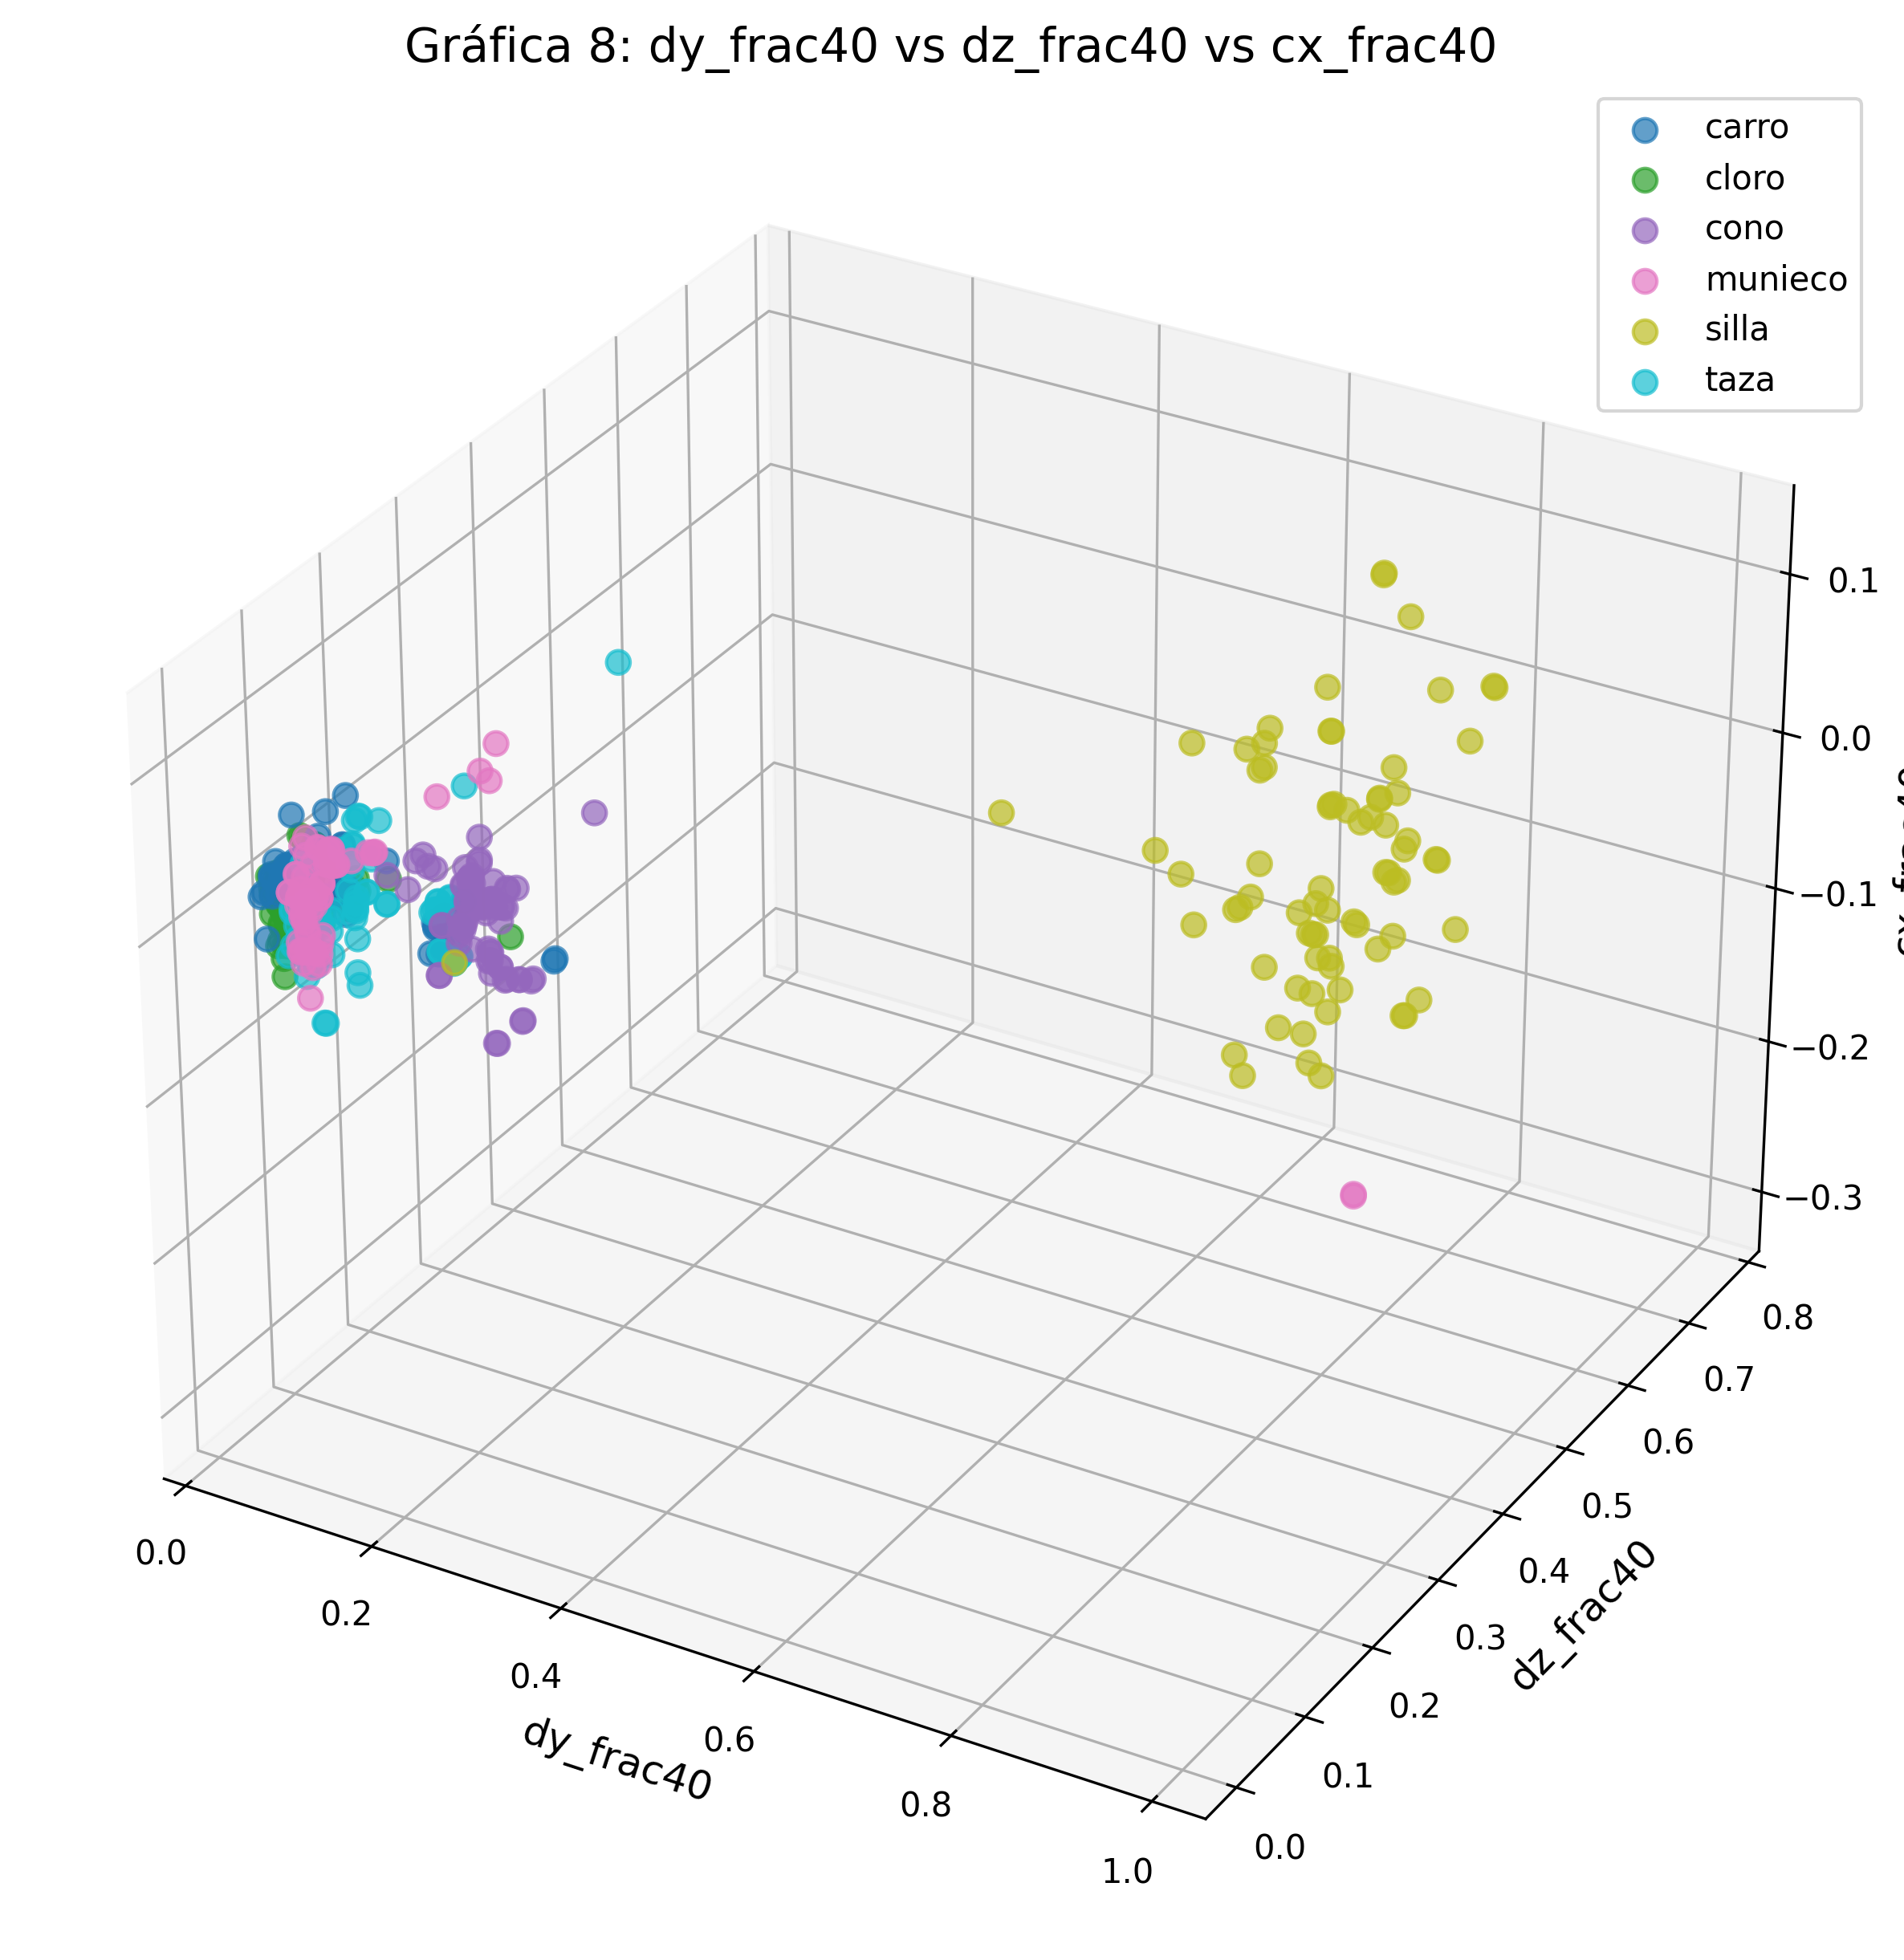
\includegraphics{images/variables/grafica_combinada_08.png}} \\
        \hline
        cy\_frac40, cz\_frac40, curvature\_frac40 & 
        \adjustbox{max width=\linewidth,max height=3cm}{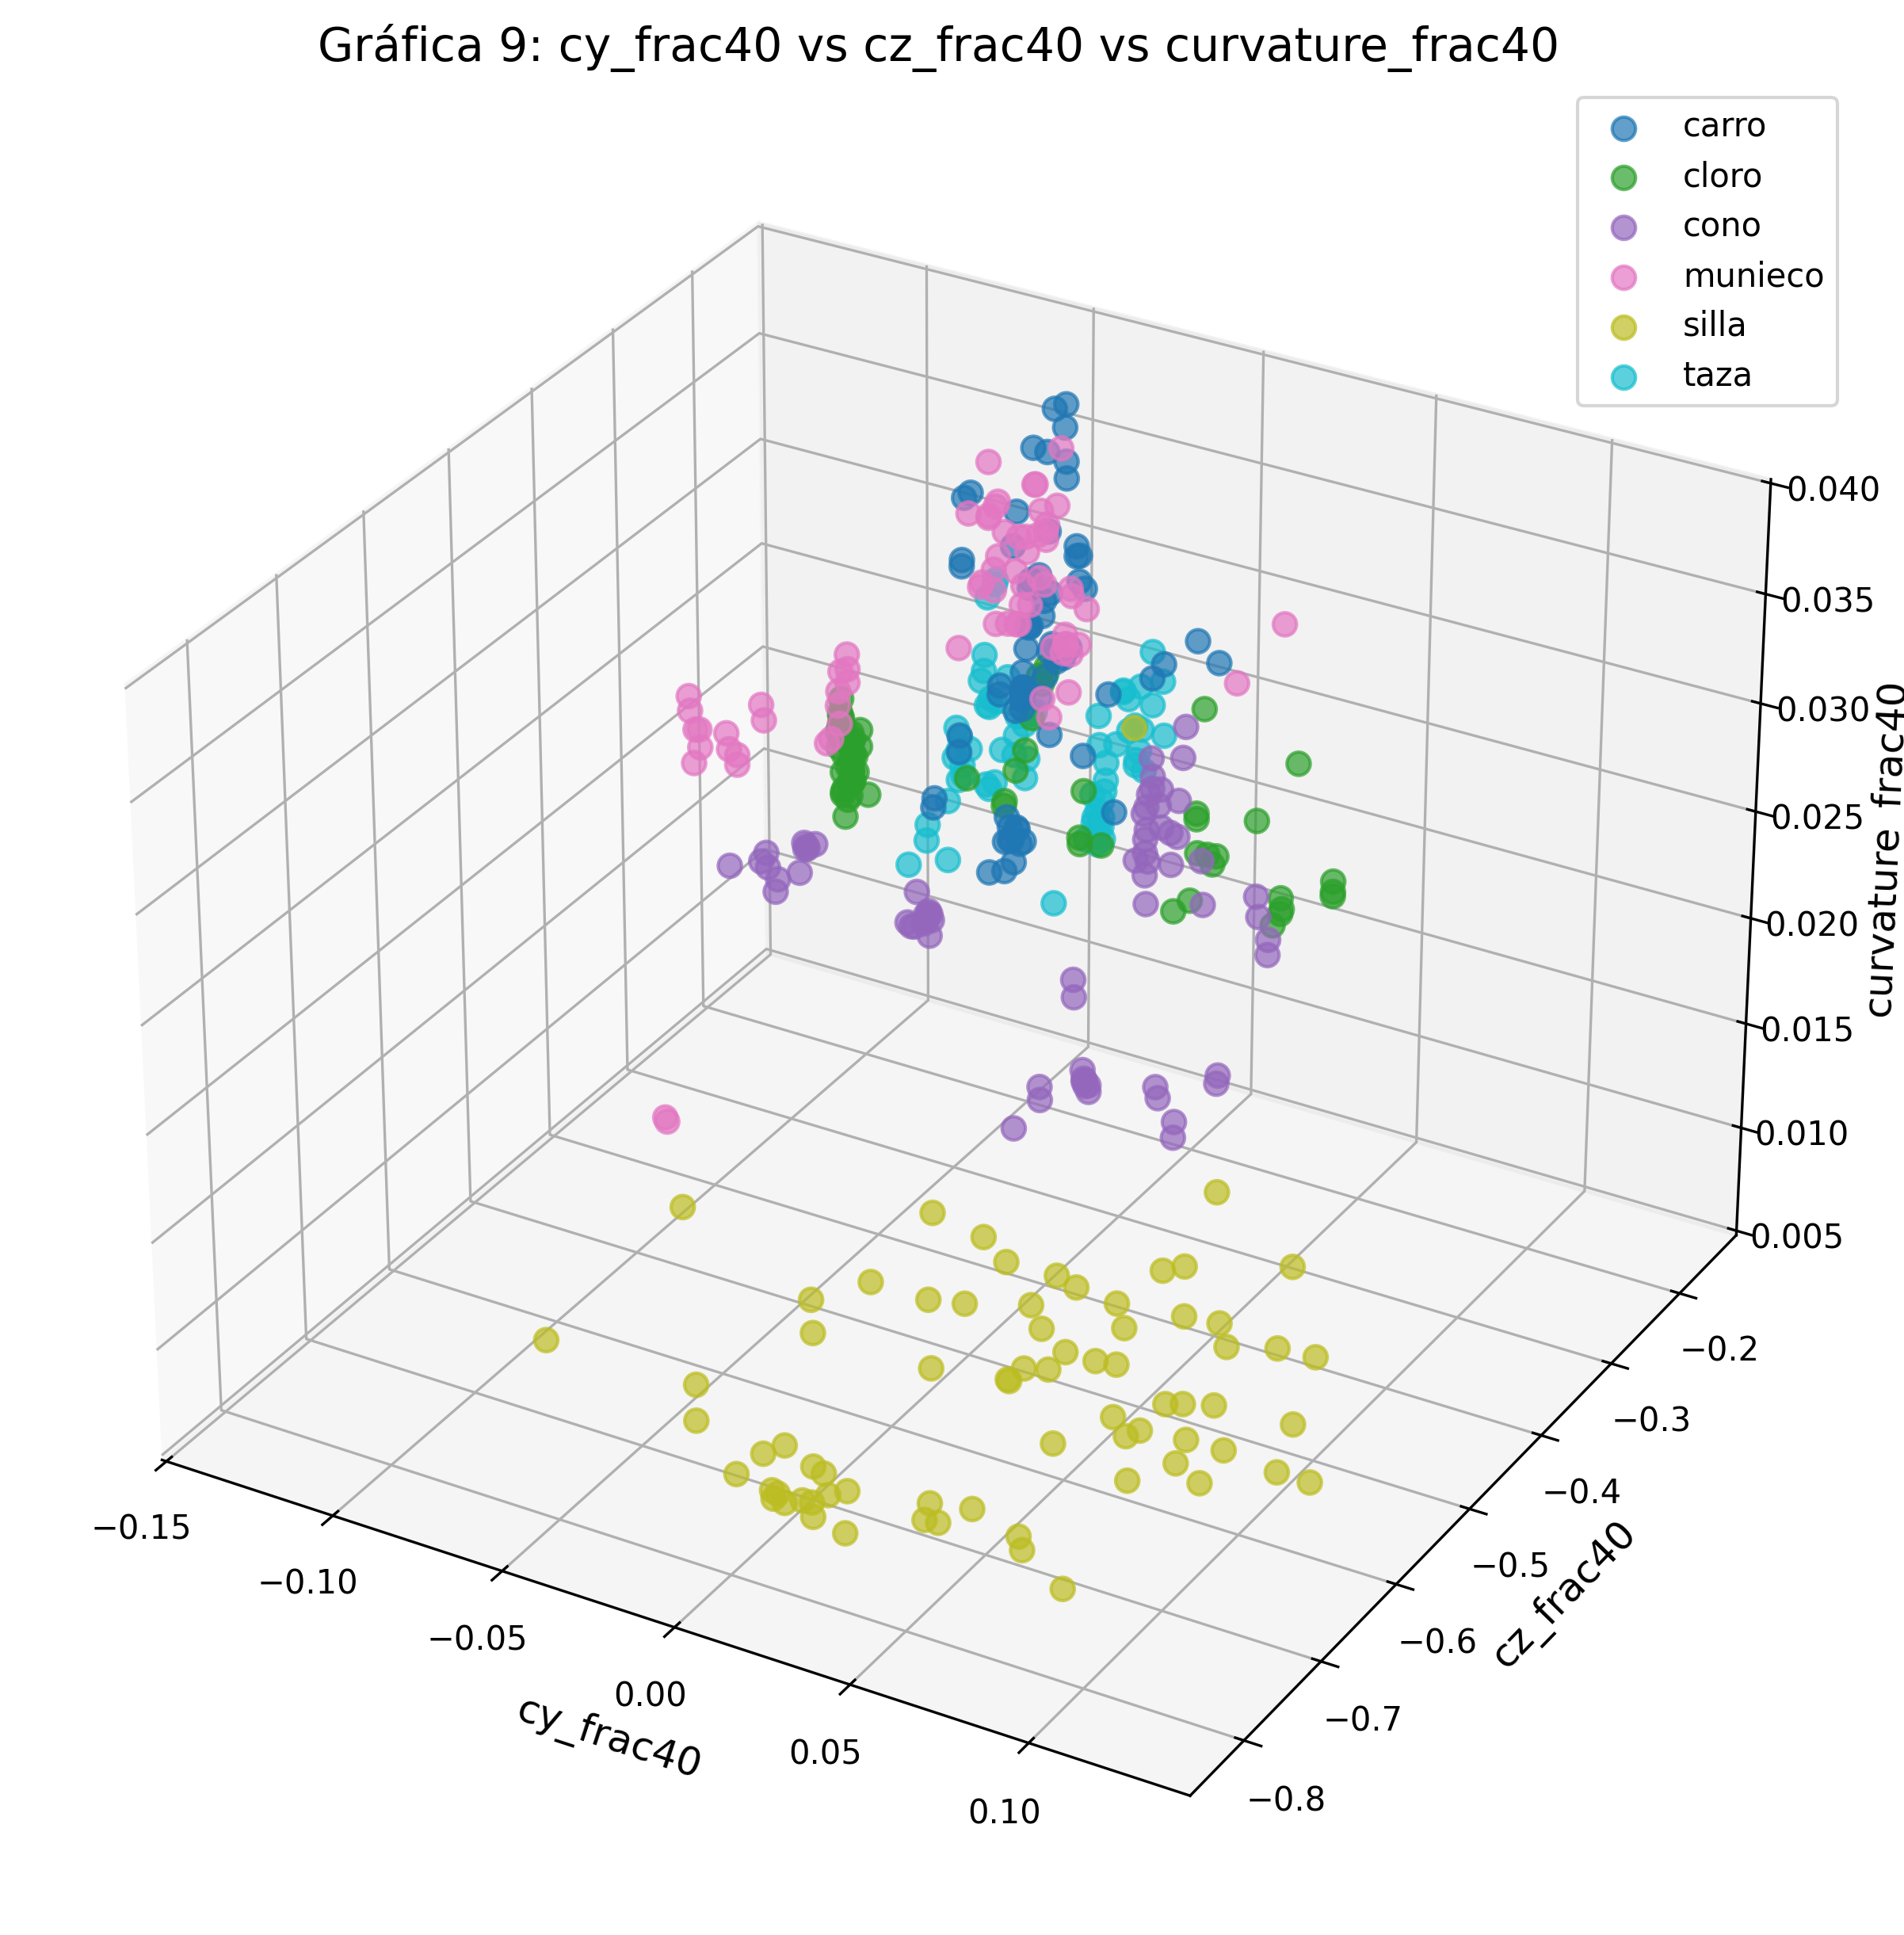
\includegraphics{images/variables/grafica_combinada_09.png}} \\
        \hline
        border\_frac40, compacidad\_frac40, fpfh\_frac40 & 
        \adjustbox{max width=\linewidth,max height=3cm}{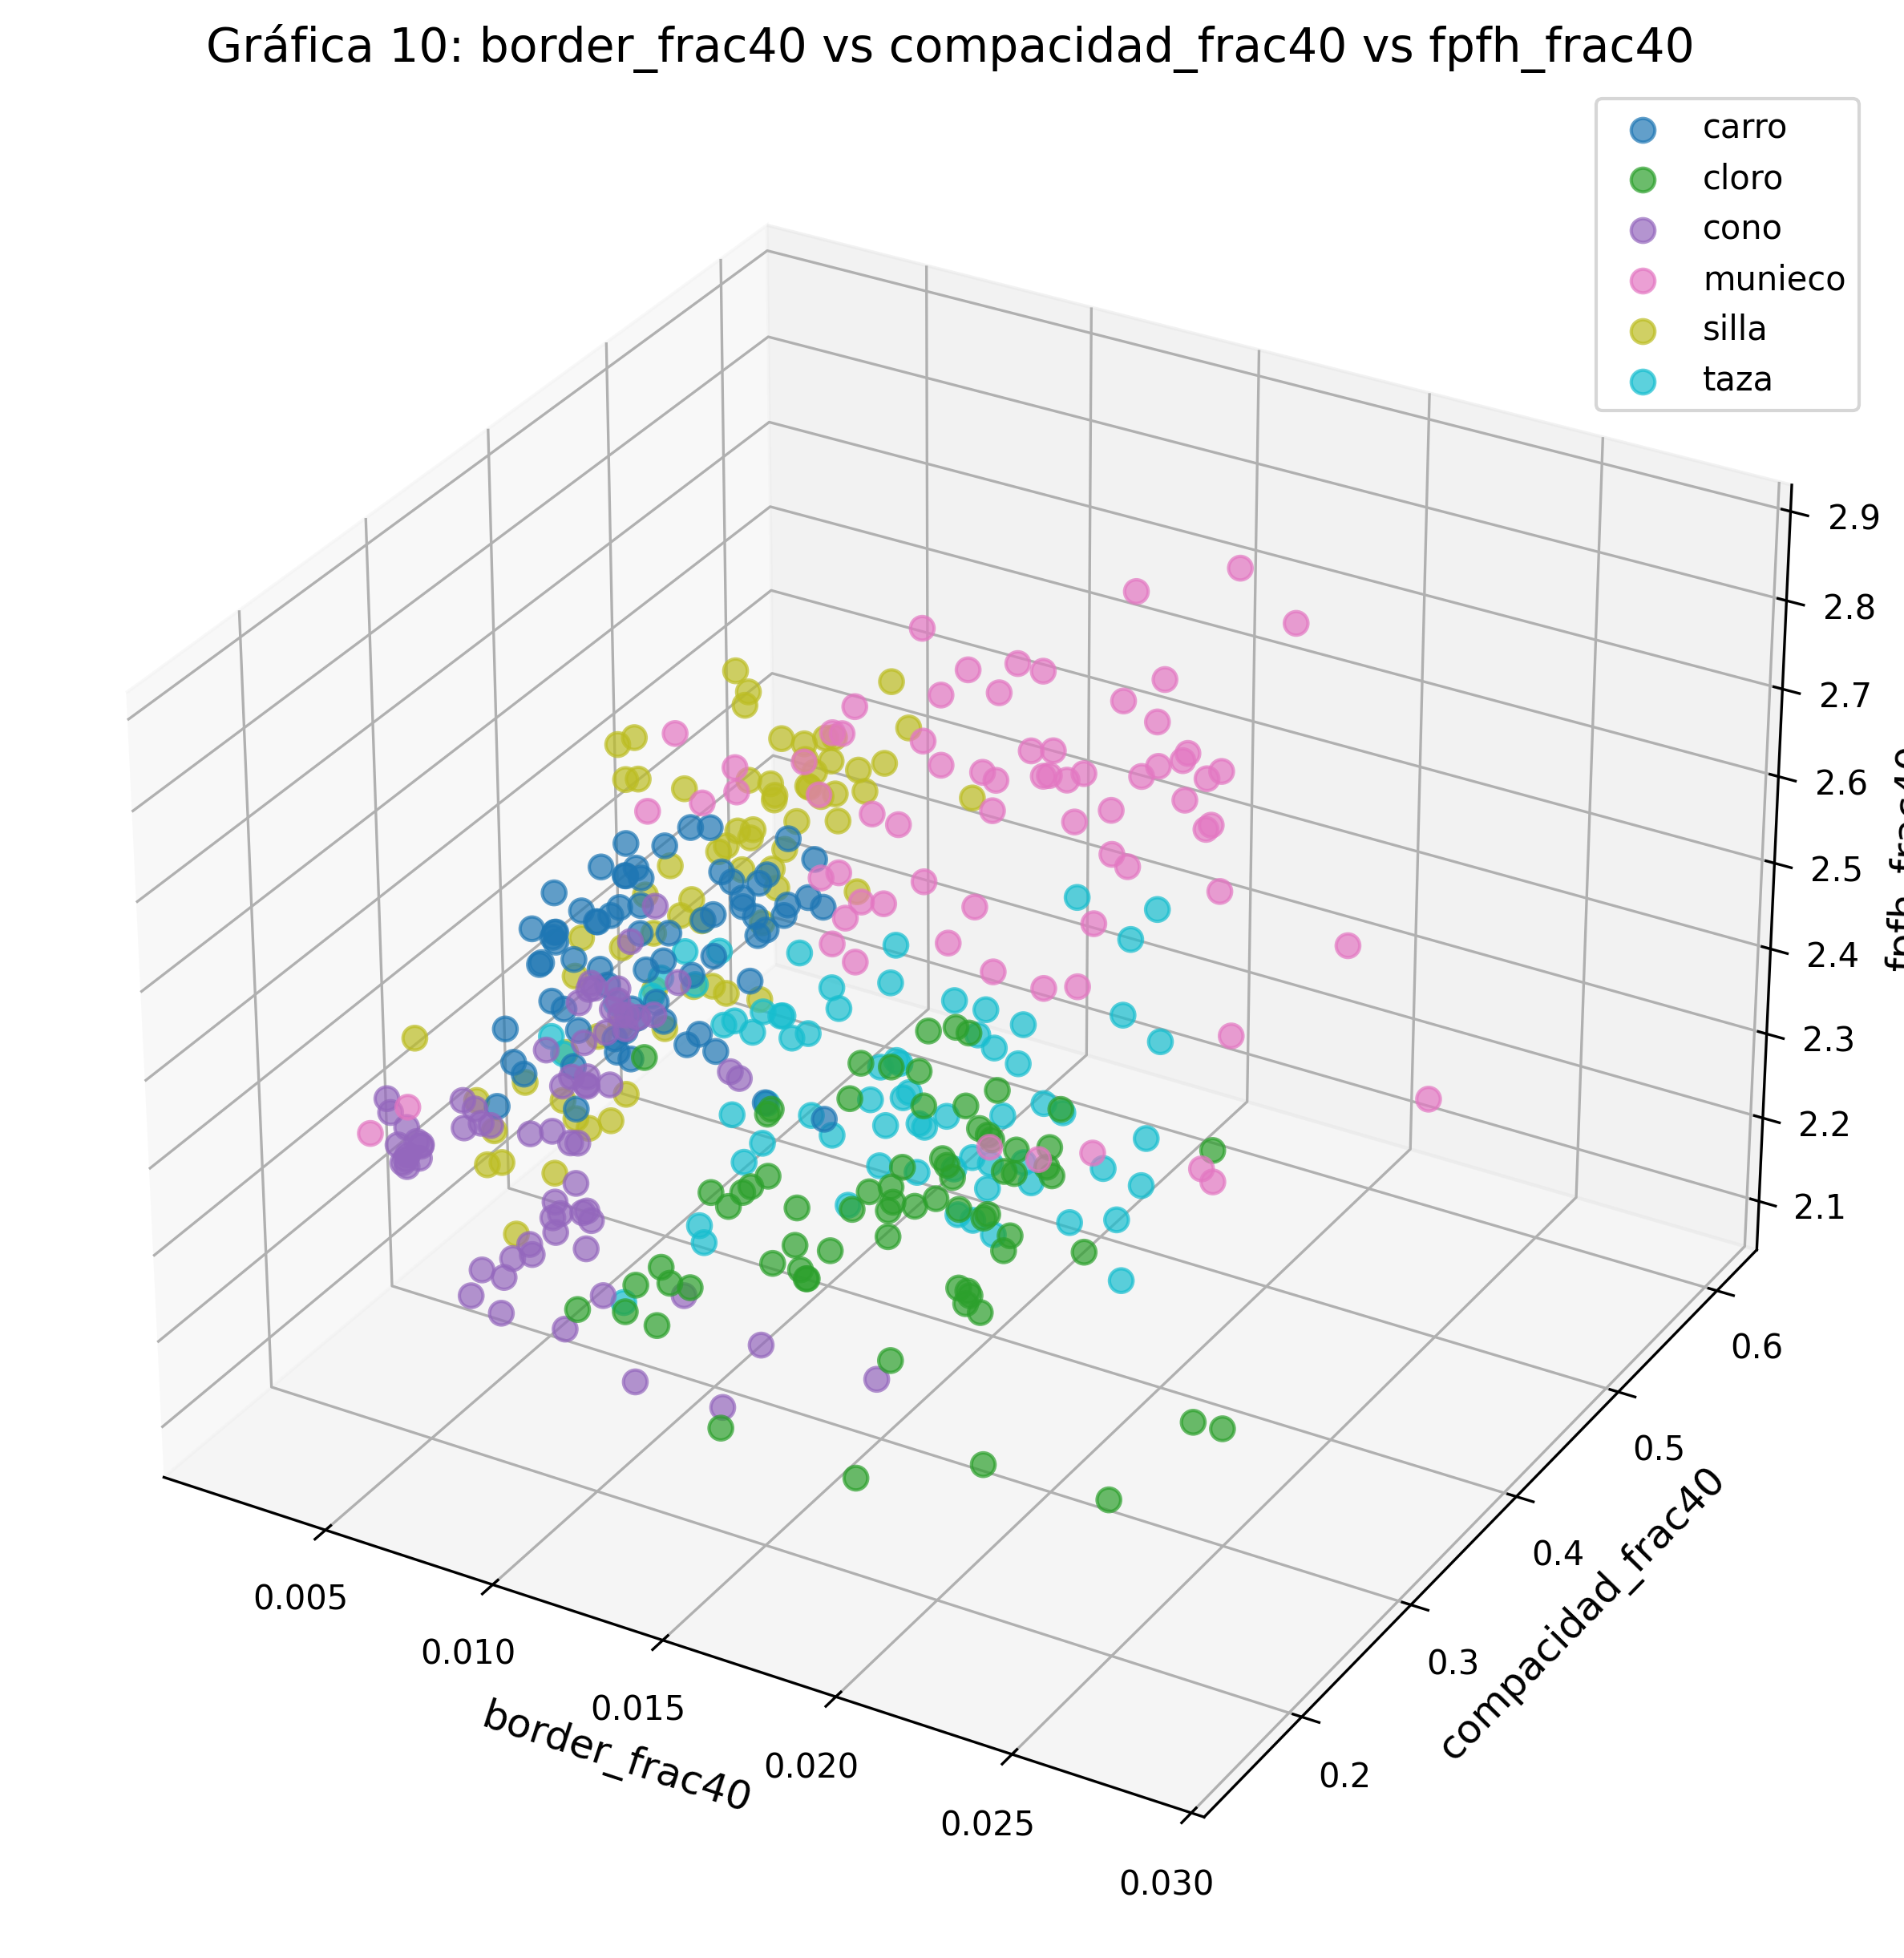
\includegraphics{images/variables/grafica_combinada_10.png}} \\
        \hline
        dx\_frac50, dy\_frac50, dz\_frac50 & 
        \adjustbox{max width=\linewidth,max height=3cm}{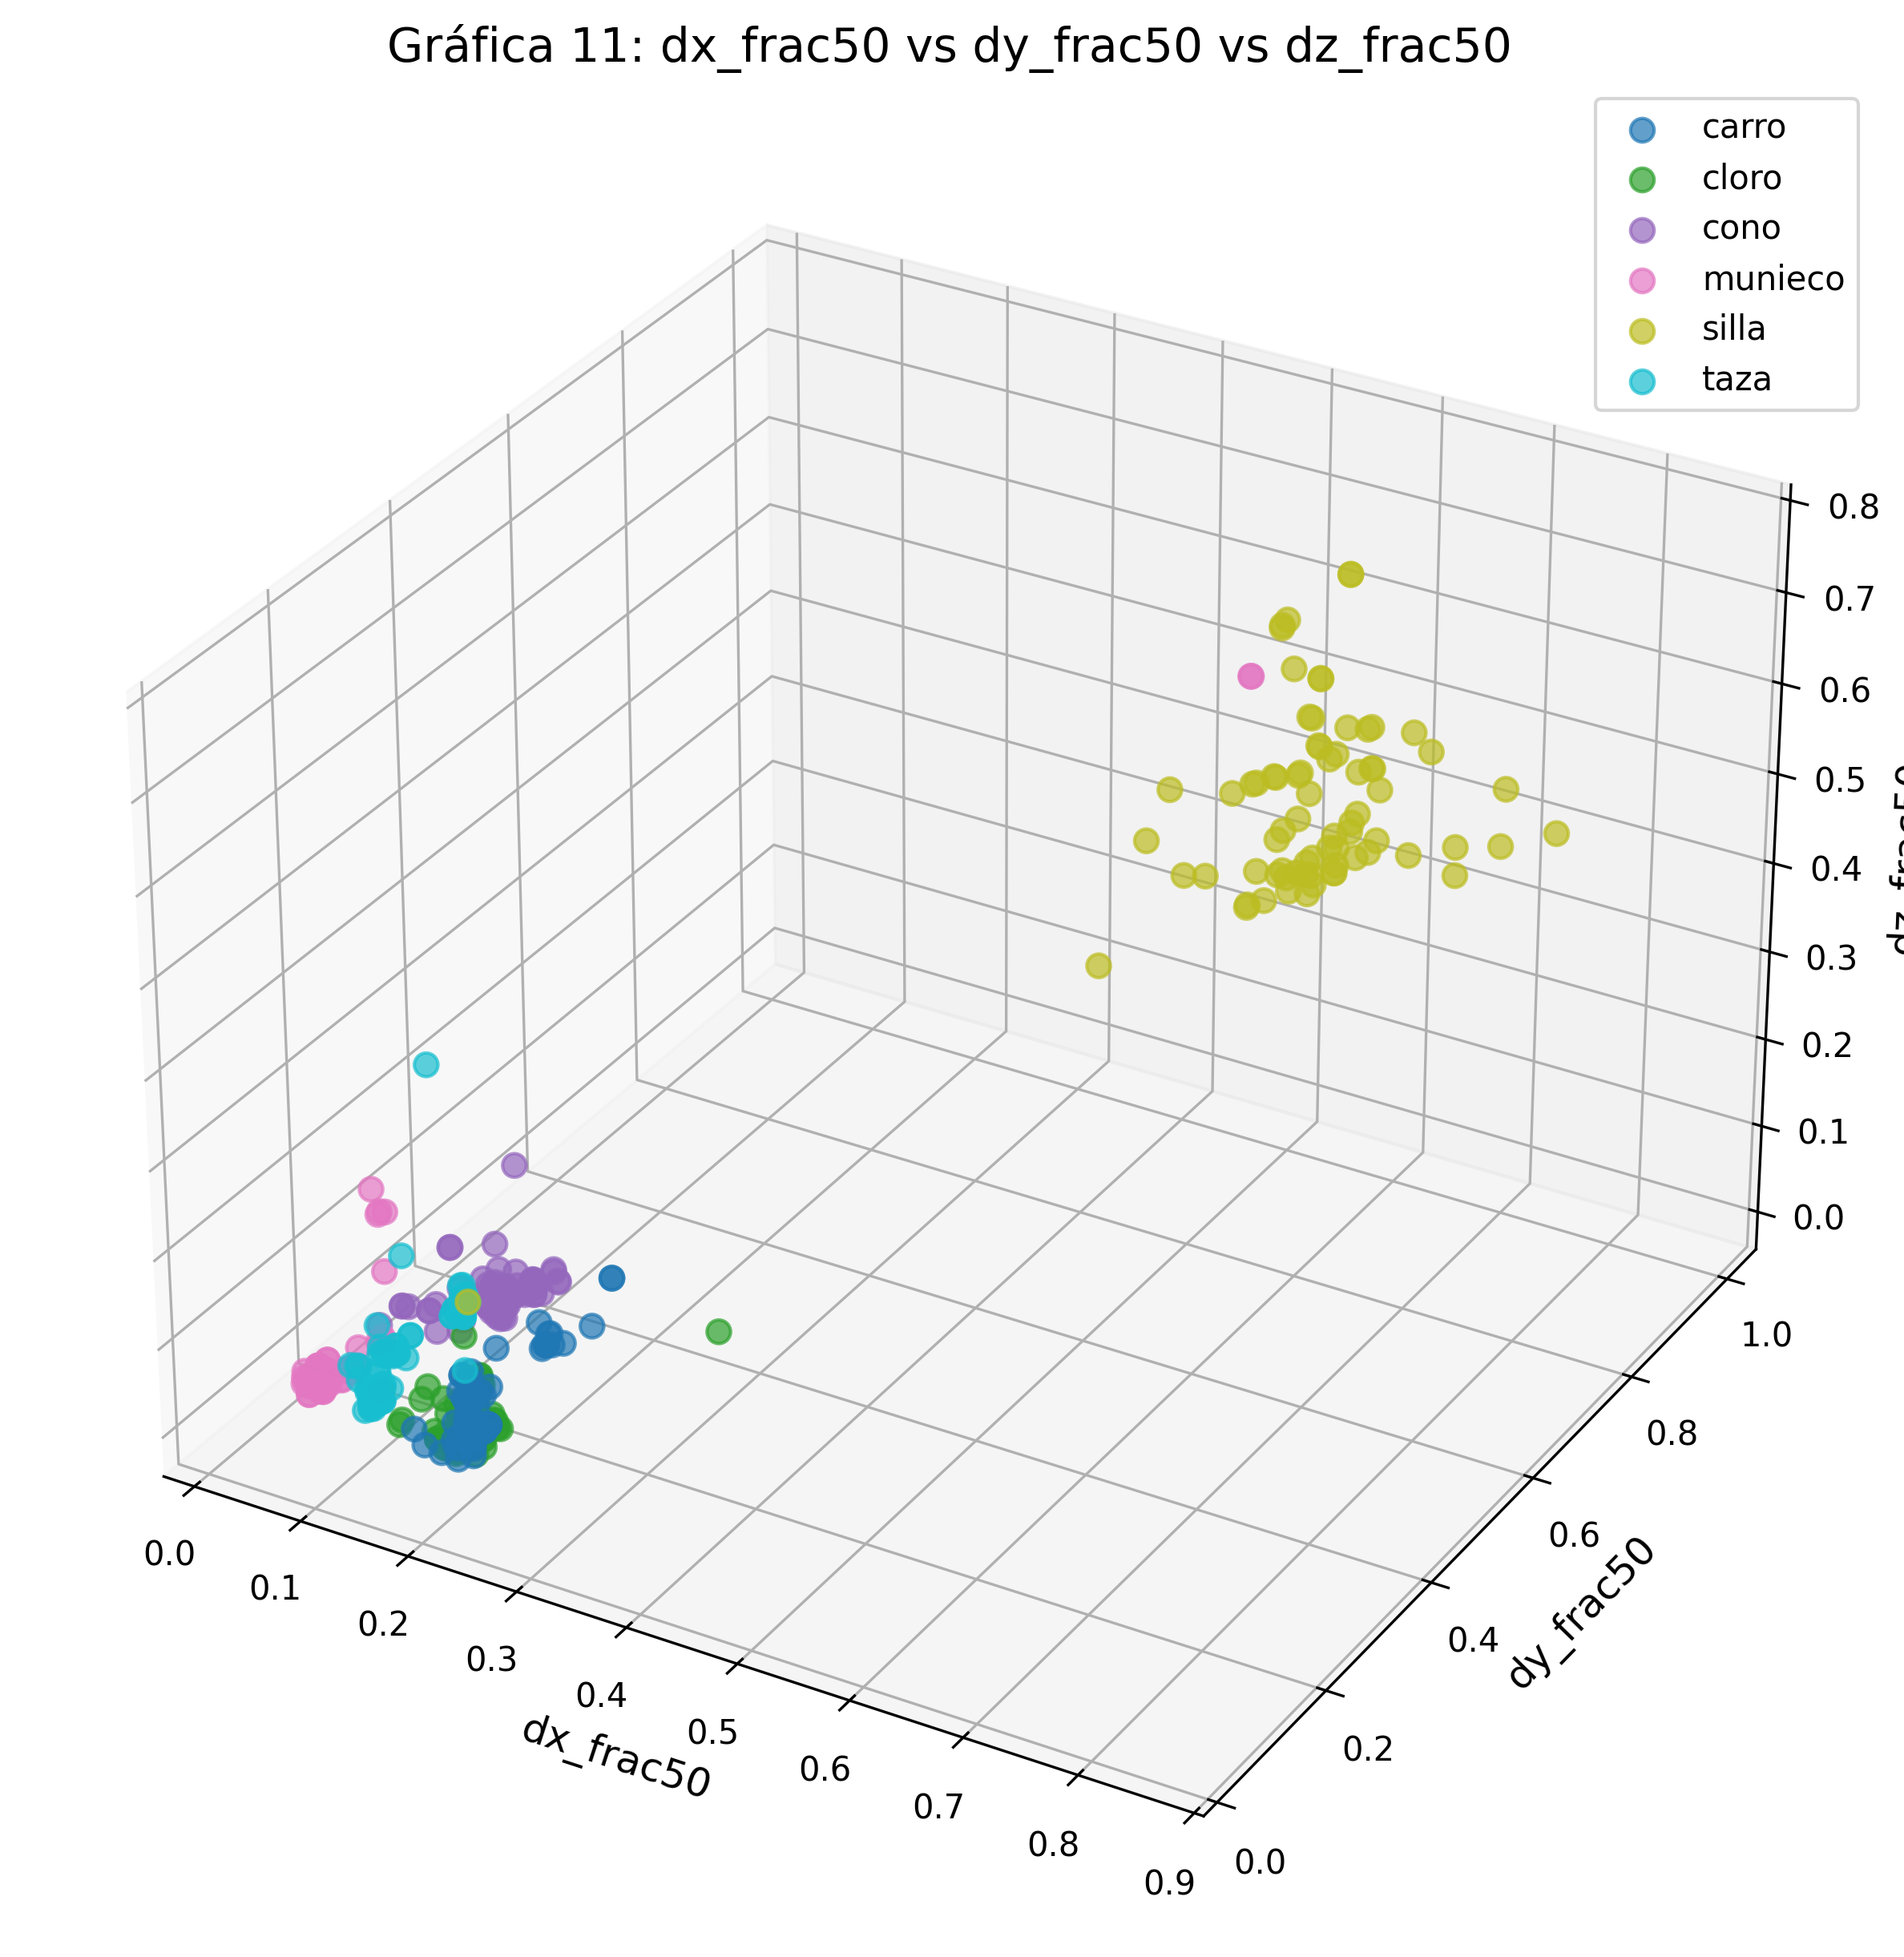
\includegraphics{images/variables/grafica_combinada_11.png}} \\
      
        \hline
        cx\_frac50, cy\_frac50, cz\_frac50 & 
        \adjustbox{max width=\linewidth,max height=3cm}{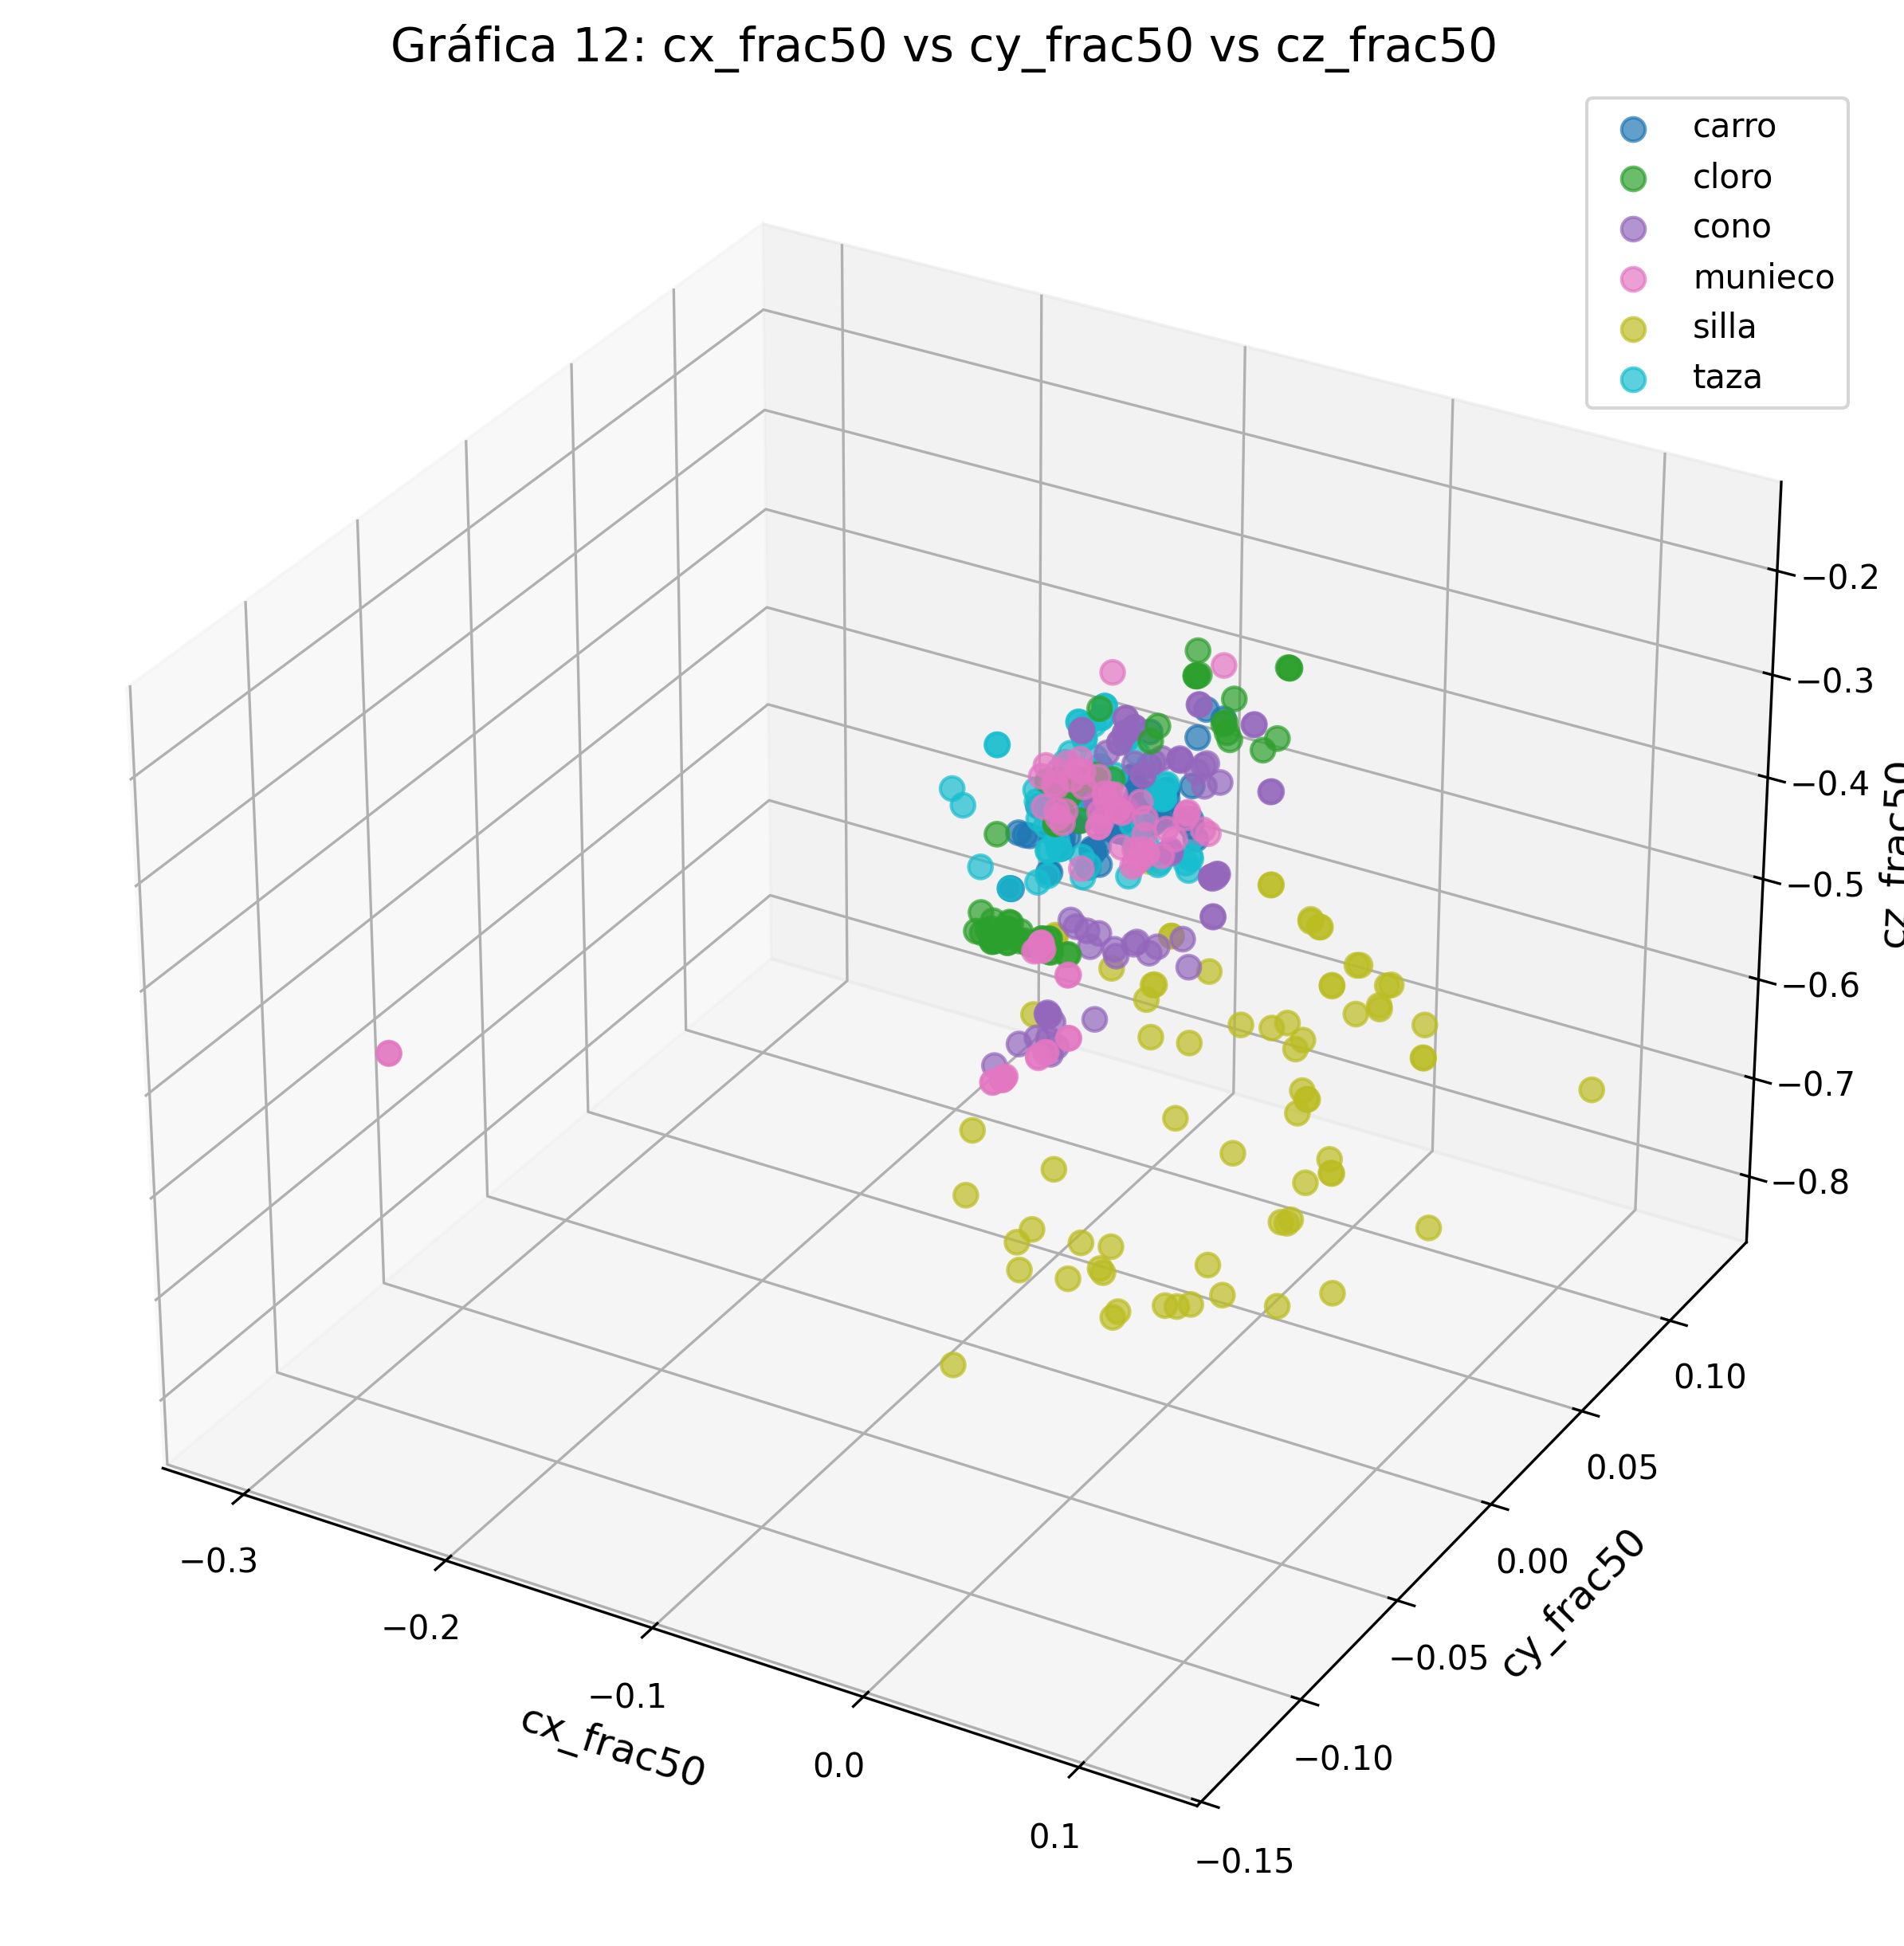
\includegraphics{images/variables/grafica_combinada_12.png}} \\
        \hline
        curvature\_frac50, border\_frac50, compacidad\_frac50 & 
        \adjustbox{max width=\linewidth,max height=3cm}{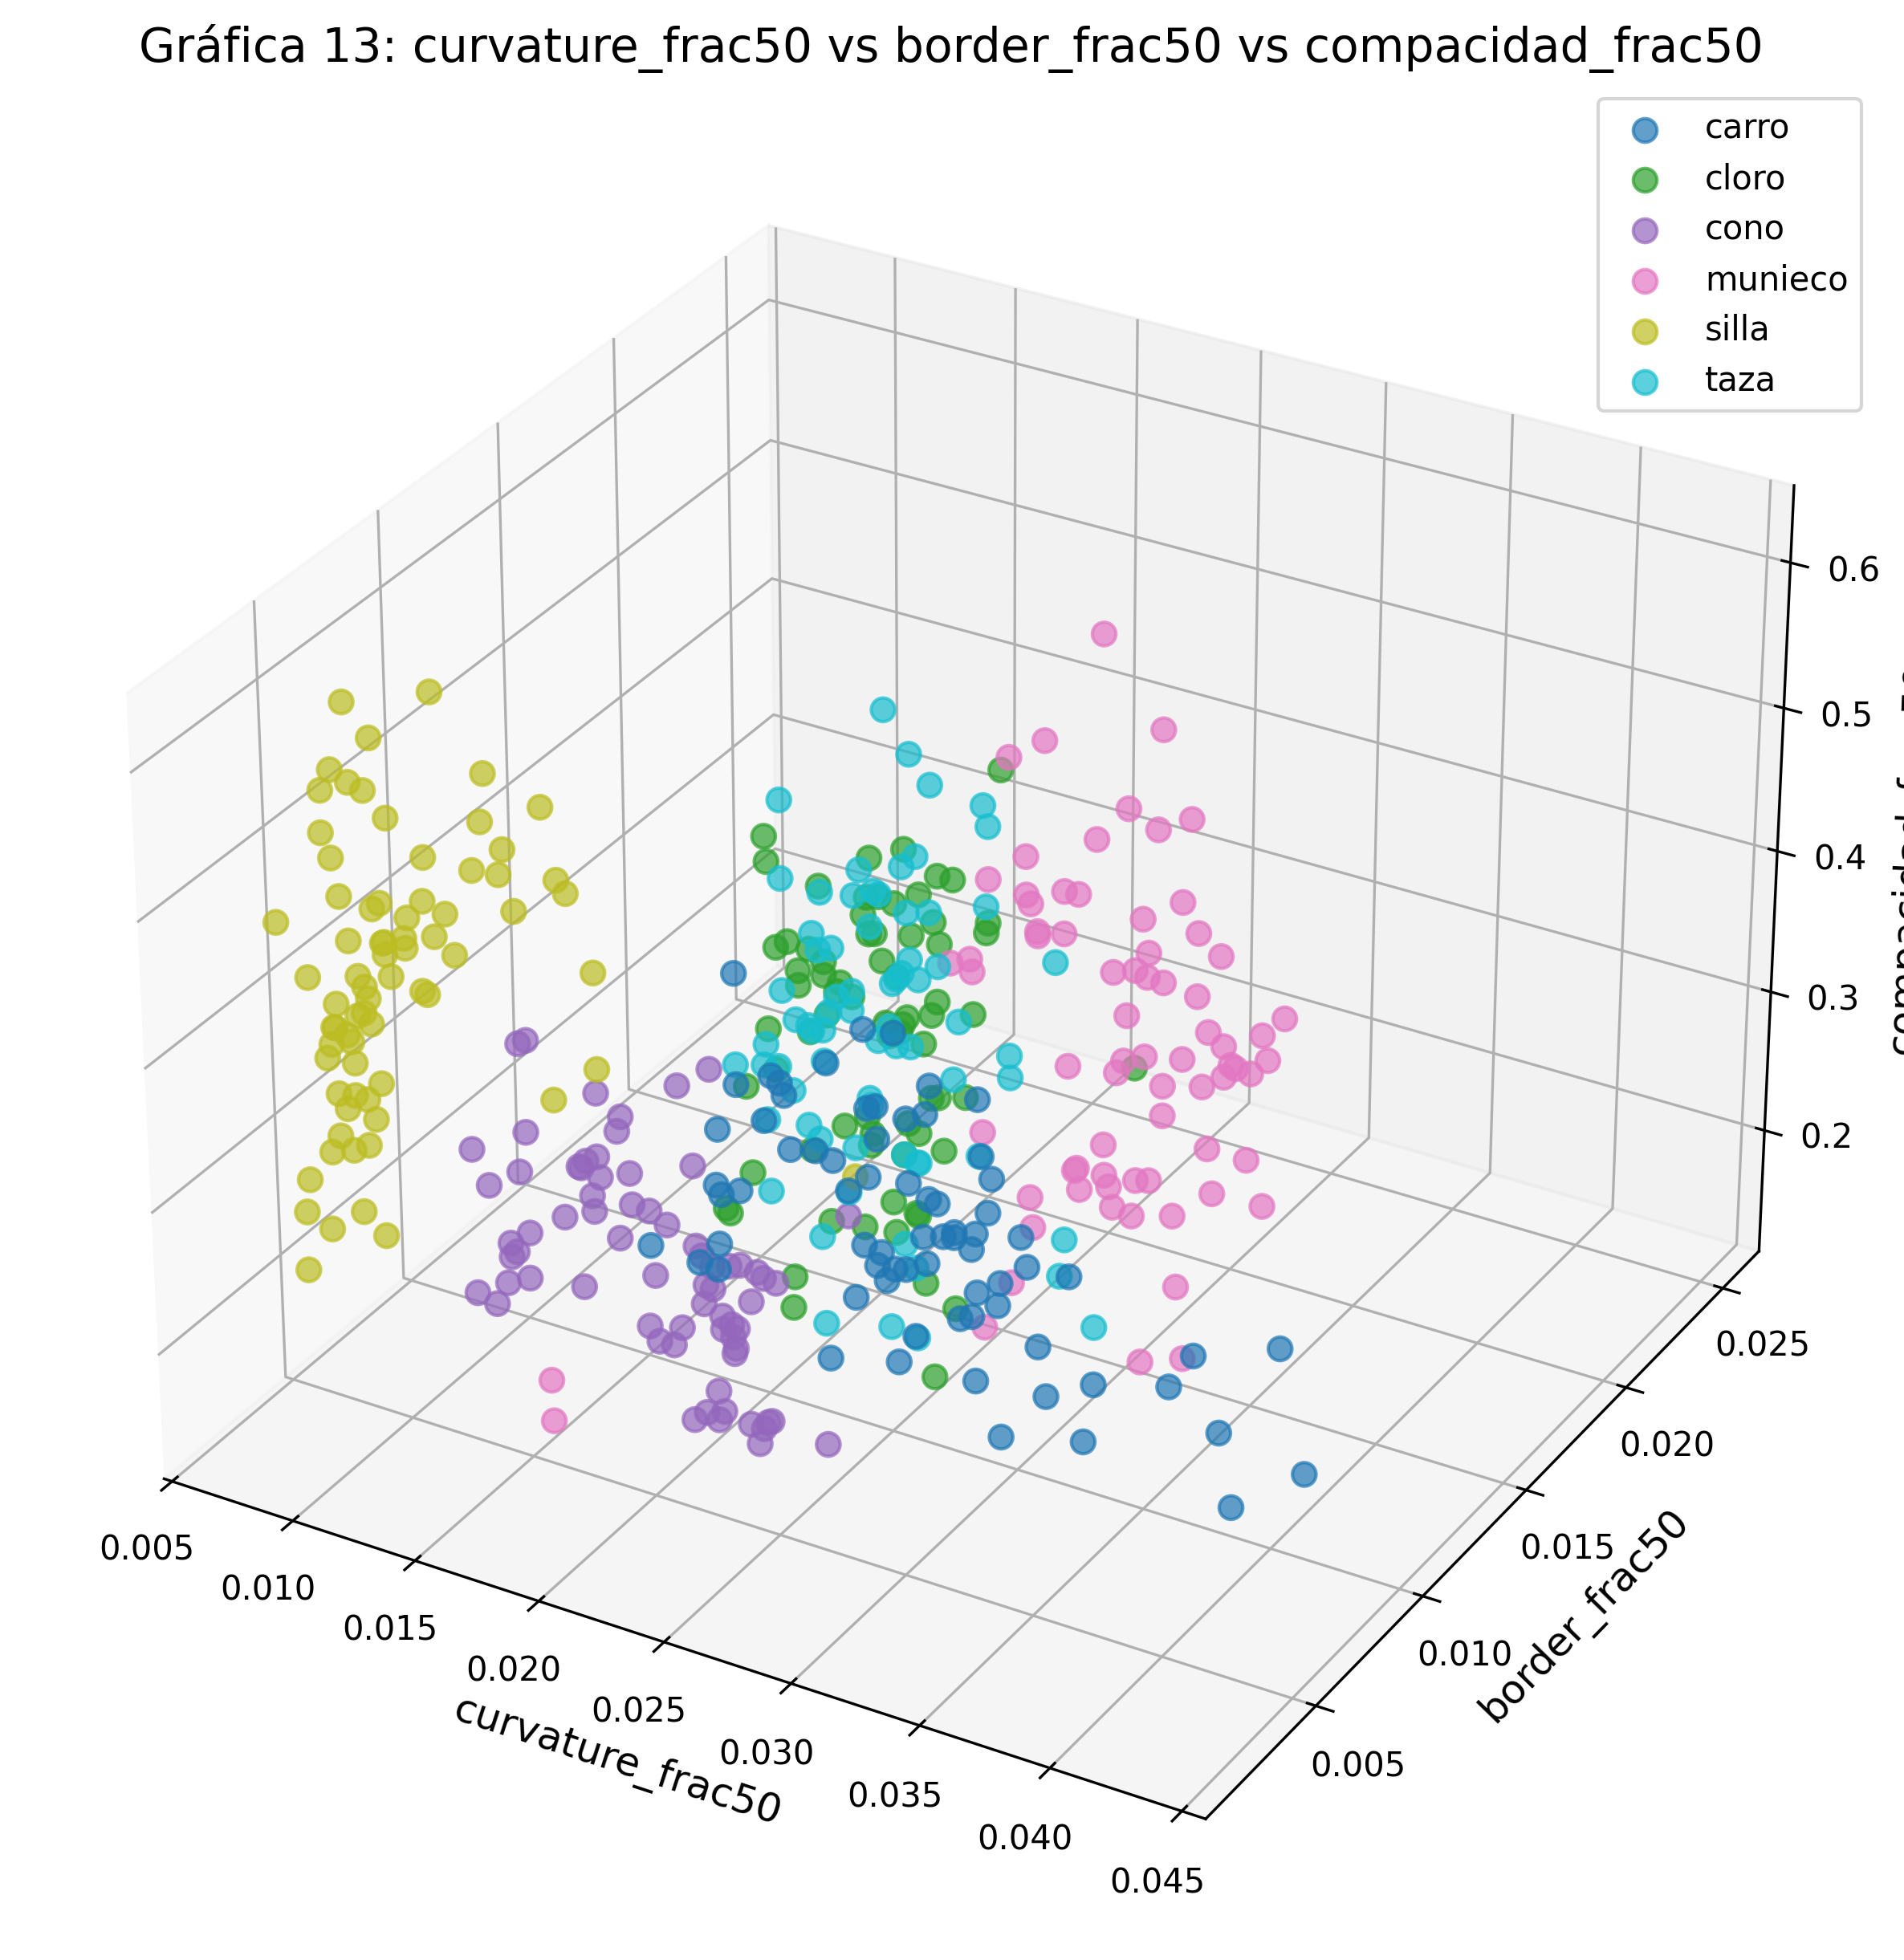
\includegraphics{images/variables/grafica_combinada_13.png}} \\
        
    \end{tabular}
\end{table}
Cada color representa una clase o categoría y cada clase posee su propio punto. Dentro de las dimensiones podemos ver cada una de las variables. Con esto podemos ver que en algunas variables existe un abismal marco de diferencia, mientras que en otras solo existe una pequeña. Pero prestese atención a la del cloro y carro,(verde y azul marino respectivamente), ya que algunas de sus características se sobreponen. Esto nos podría dar indicios que posiblemente vayan a haber predicciones erróneas en base a esas dos categorías.
\subsection{Árbol de decisiones}
Las pruebas se realizaron antes que el último compañero colocará sus datos, por lo tanto habían 6 compañeros que subieron sus categorías.
El árbol de decisión se basa en generar un conjunto de condiciones en las que las características puedan entrar, generar posibles vías y de las cuales, permitirán el proceso de clasificación debido a que podrá encontrar las características que puedan determinar si pertenece o no a una categoría.
Para entrenar el árbol se utiliza la librería de scikit learn, que ya posee el modelo construido, a su vez de que posee los hiperpárametros para ser ajustados. Además en Scikit learn, posee funciones para calcular métricas, que será accuracy, f1 score, recall y precision. También con la ayuda de seaborns, se puede generar un gráfico del tipo heat map, para observar las categorías ya clasificados y cuales fueron falsos y verdaderos positivos. Antes de entrenar el árbol primero hay que dividir el conjunto de datos, ya se como entrada salida tanto para valores de entrada numérica como para las categorías, o un cross validation. En este caso y por simpleza se escoge la clásica división entrenamiento y prueba. 
Cuando se termina de entrenar, se utiliza  otro modulo de scikit denominado \textit{learning rate}, del cual realiza un cross validation y se le pasa tanto el modelo como datos dfe entrenamiento
Se va a comparar en cuestión de resultados además, lo que salió con este conjunto y con el conjunto de los demás.
\section{Resultados}
La prueba se realizo con los parámetros y accuracies que se muestran en la tabla \ref{tab:comparacion_modelos_dt} y en la tabla \ref{tab:comparacion_learning} se muestra el mapa de clasificación y la curva de aprendizaje. Al principio indica una sobreajuste claro, ya que se ve la línea de la muerte , pero conforme va aumentando la cantidad de datos, la curva para test aumenta y la de train baja. De esta manera, se ve que la diferencia entre las dos decrementa y llega a un punto convergente.  Un problema que se visualizo es que al dividir con train split,no daba las clases balanceadas, esto es debido a que cuando se hace el split, da número fraccionario. Por lo que se realizó el proceso manual de selección de filas o datos. El mínimo de clases que se mostraba en el balance es de 21, por lo que se busca que todas las clases puedan tener esos 21 elementos.
Para evaluarlo se utilizarán métricas como accuracy, precision, recall y f1\-score
\begin{table}[h]
    \centering
    \caption{Comparación de modelos DecisionTreeClassifier con diferentes parámetros}
    \label{tab:comparacion_modelos_dt}
    \setlength{\tabcolsep}{4pt}
    \renewcommand{\arraystretch}{1.3}
    \begin{tabular}{|>{\centering\arraybackslash}m{0.48\columnwidth}|
                    >{\arraybackslash}m{0.48\columnwidth}|}
        \hline
        \textbf{Parámetros del modelo} & \textbf{Resultados} \\
        \hline
        \texttt{max\_depth=5, min\_samples\_split=5, ccp\_alpha=0.001, criterion=gini} &
        Train Acc: 0.970 \newline 
        Test Acc: 0.960 \newline 
        Diferencia: 0.010 \newline 
        Macro avg: Prec=0.96, Rec=0.96, F1=0.96 \\
        \adjustbox{max width=\linewidth,max height=3cm}{\includegraphics{images/}} \\
        \hline
        \texttt{max\_depth=5, min\_samples\_split=5, ccp\_alpha=0.001, criterion=entropy} &
        Train Acc: 0.997 \newline 
        Test Acc: 0.873 \newline 
        Diferencia: 0.124 \newline 
        Macro avg: Prec=0.92, Rec=0.87, F1=0.86 \\
        \hline
        \texttt{max\_depth=5, min\_samples\_split=5, ccp\_alpha=0.001, criterion=log\_loss} &
        Train Acc: 0.997 \newline 
        Test Acc: 0.873 \newline 
        Diferencia: 0.124 \newline 
        Macro avg: Prec=0.92, Rec=0.87, F1=0.86 \\
        \hline
        \texttt{max\_depth=5, min\_samples\_split=5, ccp\_alpha=0.005, criterion=gini} &
        Train Acc: 0.971 \newline 
        Test Acc: 0.960 \newline 
        Diferencia: 0.010 \newline 
        Macro avg: Prec=0.96, Rec=0.96, F1=0.96 \\
        \hline
        \texttt{max\_depth=4, min\_samples\_split=5, ccp\_alpha=0.005, criterion=gini} &
        Train Acc: 0.941 \newline 
        Test Acc: 0.937 \newline 
        Diferencia: 0.005 \newline 
        Macro avg: Prec=0.94, Rec=0.94, F1=0.94 \\
        \hline
    \end{tabular}
\end{table}
\begin{table}[h!]
    \centering
    \caption{Comparación de modelos DecisionTreeClassifier con diferentes parámetros}
    \label{tab:comparacion_learning}
    \setlength{\tabcolsep}{4pt}
    \renewcommand{\arraystretch}{1.3}
    \begin{tabular}{|>{\centering\arraybackslash}m{0.32\columnwidth}|
                    >{\centering\arraybackslash}m{0.32\columnwidth}|
                    >{\centering\arraybackslash}m{0.32\columnwidth}|}
        \hline
        \textbf{Parámetros del modelo} & \textbf{Heat map} & \textbf{Curva de aprendizaje} \\
        \hline
        \texttt{max\_depth=5, min\_samples\_split=5, ccp\_alpha=0.001, criterion=gini} &
        \adjustbox{max width=\linewidth,max height=3cm}{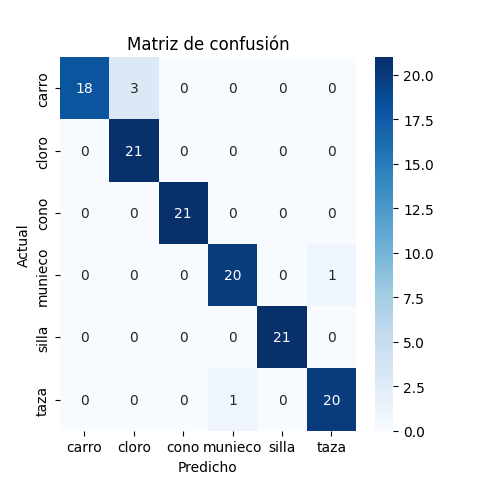
\includegraphics{images/plots/heat_map.png}} &
        \adjustbox{max width=\linewidth,max height=3cm}{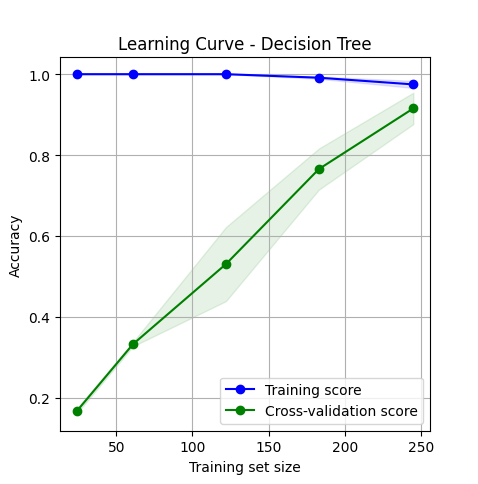
\includegraphics{images/plots/learning_curve.png}} \\
        \hline
        \texttt{max\_depth=5, min\_samples\_split=5, ccp\_alpha=0.001, criterion=entropy} &
        \adjustbox{max width=\linewidth,max height=3cm}{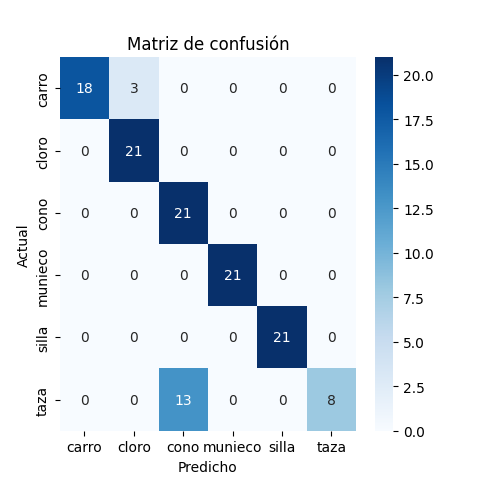
\includegraphics{images/plots/heat_map_1.png}} &
        \adjustbox{max width=\linewidth,max height=3cm}{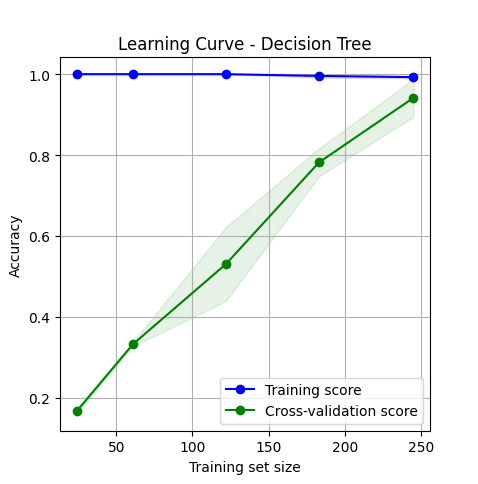
\includegraphics{images/plots/learning_curve_1.png}} \\
        \hline
        \texttt{max\_depth=5, min\_samples\_split=5, ccp\_alpha=0.001, criterion=log\_loss} &
        \adjustbox{max width=\linewidth,max height=3cm}{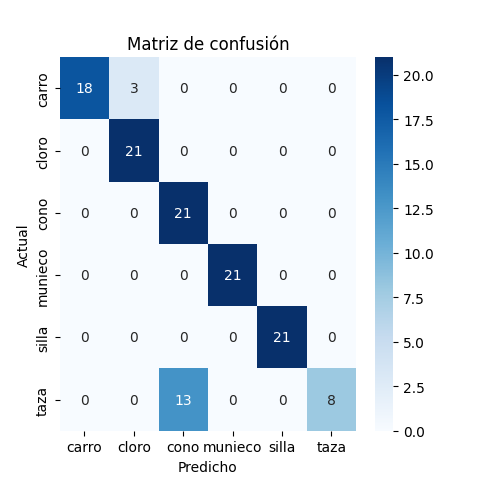
\includegraphics{images/plots/heat_map_2.png}} &
        \adjustbox{max width=\linewidth,max height=3cm}{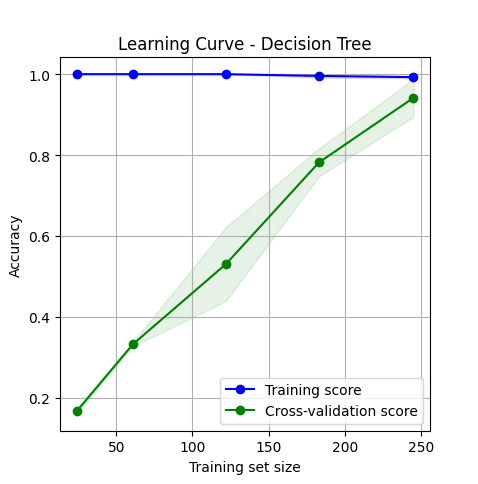
\includegraphics{images/plots/learning_curve_2.png}} \\
        \hline
        \texttt{max\_depth=5, min\_samples\_split=5, ccp\_alpha=0.005, criterion=gini} &
        \adjustbox{max width=\linewidth,max height=3cm}{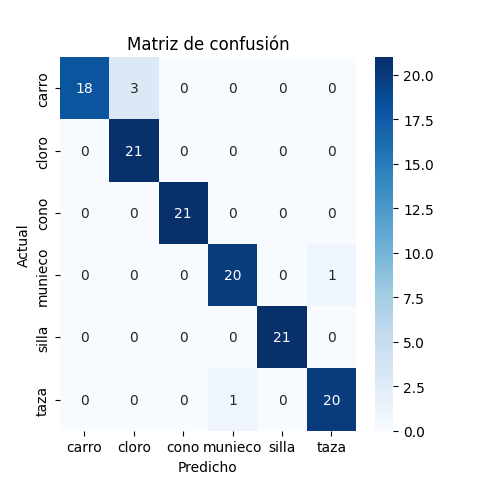
\includegraphics{images/plots/heat_map_3.png}} &
        \adjustbox{max width=\linewidth,max height=3cm}{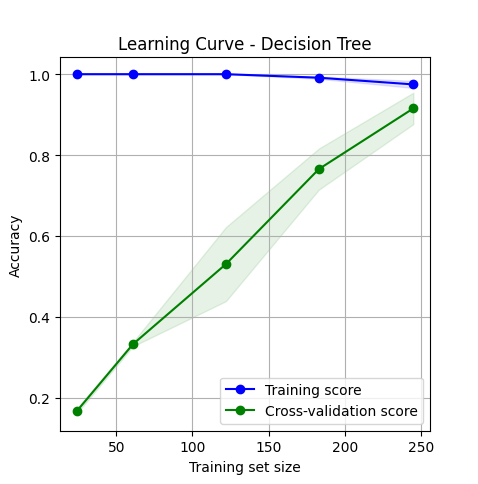
\includegraphics{images/plots/learning_curve_3.png}} \\
        \hline
        \texttt{max\_depth=4, min\_samples\_split=5, ccp\_alpha=0.005, criterion=gini} &
        \adjustbox{max width=\linewidth,max height=3cm}{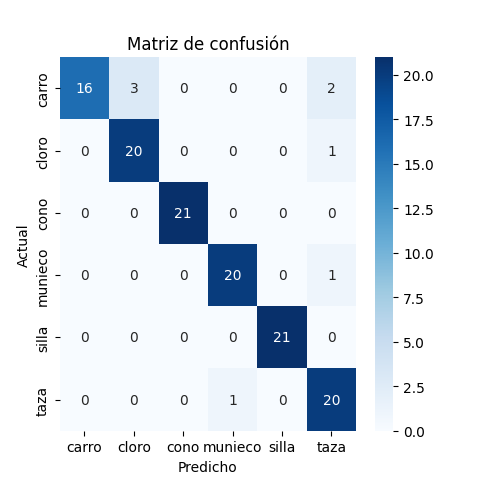
\includegraphics{images/plots/heat_map_4.png}} &
        \adjustbox{max width=\linewidth,max height=3cm}{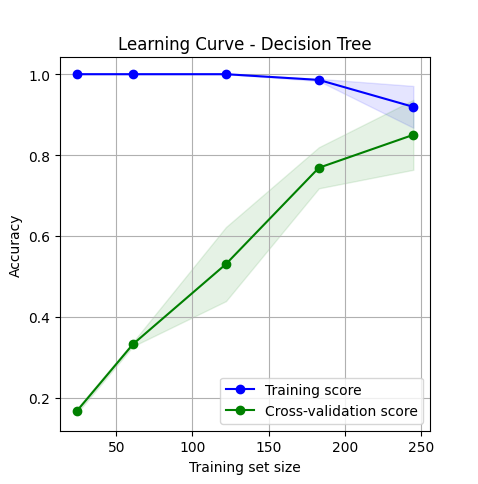
\includegraphics{images/plots/learning_curve_4.png}} \\
        \hline
    \end{tabular}
\end{table}
Ahora revisaremos con el siguiente conjunto de datos, que posee los datos del compañero por medio de las tablas \ref{tab:comparacion_modelos_dt_extra} dónde se encuentran las métricas de evaluación y en la tabla \ref{tab:comparacion_learning_extra} donde se encuentran los modelos con sus gráficos 
\begin{table}[h!]
    \centering
    \caption{Comparación de modelos DecisionTreeClassifier en el segundo conjunto de datos}
    \label{tab:comparacion_modelos_dt_extra}
    \setlength{\tabcolsep}{4pt}
    \renewcommand{\arraystretch}{1.3}
    \begin{tabular}{|>{\centering\arraybackslash}m{0.45\columnwidth}|
                    >{\arraybackslash}m{0.45\columnwidth}|}
        \hline
        \textbf{Parámetros del modelo} & \textbf{Resultados resumidos} \\
        \hline
        \texttt{max\_depth=5, min\_samples\_split=5, ccp\_alpha=0.001, criterion=gini} &
        Train Acc: 0.973 \newline 
        Test Acc: 0.952 \newline 
        Diferencia: 0.020 \newline 
        Macro avg: Prec=0.96, Rec=0.95, F1=0.95 \\
        \hline
        \texttt{max\_depth=5, min\_samples\_split=5, ccp\_alpha=0.001, criterion=entropy} &
        Train Acc: 0.997 \newline 
        Test Acc: 0.960 \newline 
        Diferencia: 0.037 \newline 
        Macro avg: Prec=0.96, Rec=0.96, F1=0.96 \\
        \hline
        \texttt{max\_depth=5, min\_samples\_split=5, ccp\_alpha=0.001, criterion=log\_loss} &
        Train Acc: 0.973 \newline 
        Test Acc: 0.952 \newline 
        Diferencia: 0.020 \newline 
        Macro avg: Prec=0.96, Rec=0.95, F1=0.95 \\
        \hline
        \texttt{max\_depth=5, min\_samples\_split=5, ccp\_alpha=0.005, criterion=gini} &
        Train Acc: 0.972 \newline 
        Test Acc: 0.952 \newline 
        Diferencia: 0.020 \newline 
        Macro avg: Prec=0.96, Rec=0.95, F1=0.95 \\
        \hline
        \texttt{max\_depth=4, min\_samples\_split=5, ccp\_alpha=0.005, criterion=gini} &
        Train Acc: 0.942 \newline 
        Test Acc: 0.921 \newline 
        Diferencia: 0.022 \newline 
        Macro avg: Prec=0.94, Rec=0.92, F1=0.92 \\
        \hline
    \end{tabular}
\end{table}


\begin{table}[h!]
    \centering
    \caption{Comparación de modelos DecisionTreeClassifier con diferentes parámetros}
    \label{tab:comparacion_learning_extra}
    \setlength{\tabcolsep}{4pt}
    \renewcommand{\arraystretch}{1.3}
    \begin{tabular}{|>{\centering\arraybackslash}m{0.32\columnwidth}|
                    >{\centering\arraybackslash}m{0.32\columnwidth}|
                    >{\centering\arraybackslash}m{0.32\columnwidth}|}
        \hline
        \textbf{Parámetros del modelo} & \textbf{Heat map} & \textbf{Curva de aprendizaje} \\
        \hline
        \texttt{max\_depth=5, min\_samples\_split=5, ccp\_alpha=0.001, criterion=gini} &
        \adjustbox{max width=\linewidth,max height=3cm}{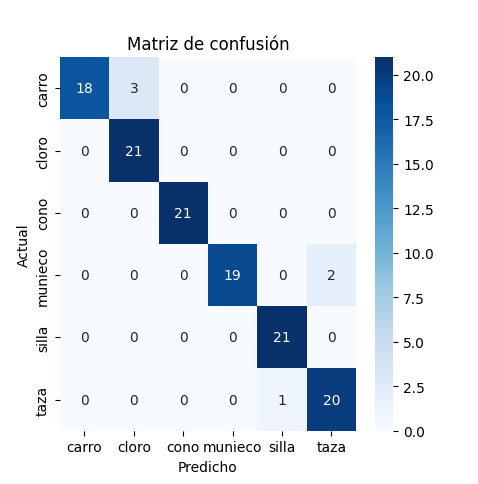
\includegraphics{images/plots/heap.png}} &
        \adjustbox{max width=\linewidth,max height=3cm}{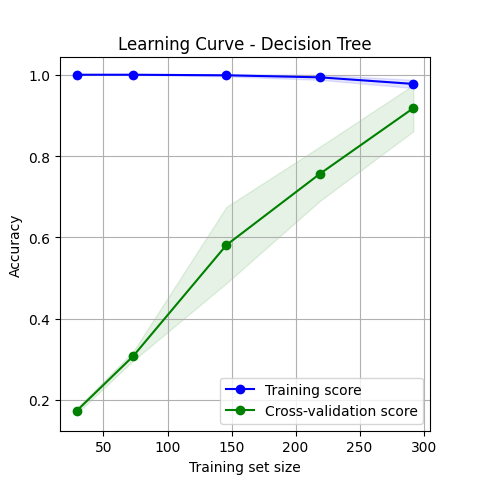
\includegraphics{images/plots/learning.png}} \\
        \hline
        \texttt{max\_depth=5, min\_samples\_split=5, ccp\_alpha=0.001, criterion=entropy} &
        \adjustbox{max width=\linewidth,max height=3cm}{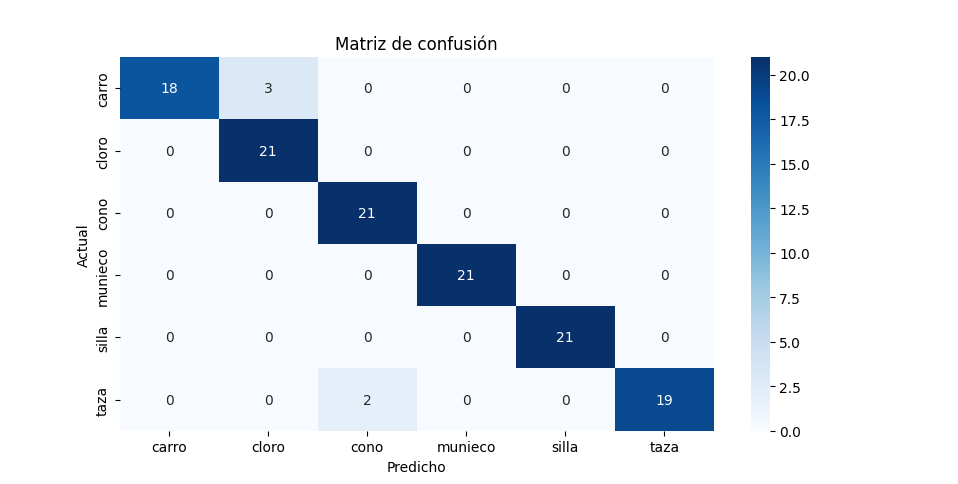
\includegraphics{images/plots/heap_1.png}} &
        \adjustbox{max width=\linewidth,max height=3cm}{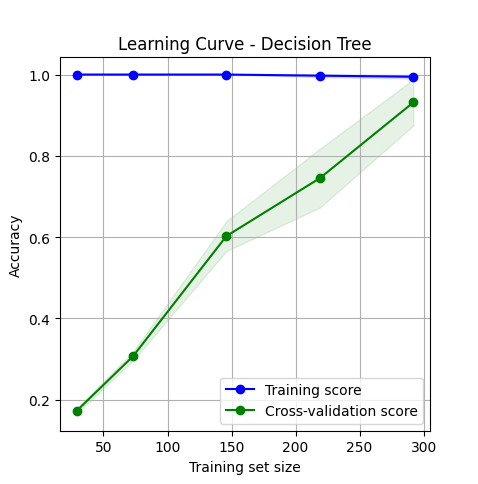
\includegraphics{images/plots/learning_1.png}} \\
        \hline
        \texttt{max\_depth=5, min\_samples\_split=5, ccp\_alpha=0.001, criterion=log\_loss} &
        \adjustbox{max width=\linewidth,max height=3cm}{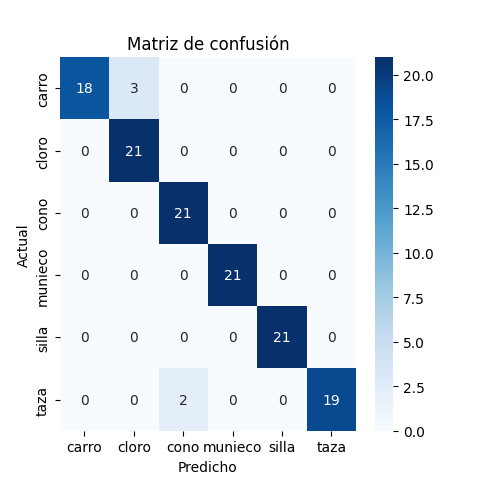
\includegraphics{images/plots/heap_2.png}} &
        \adjustbox{max width=\linewidth,max height=3cm}{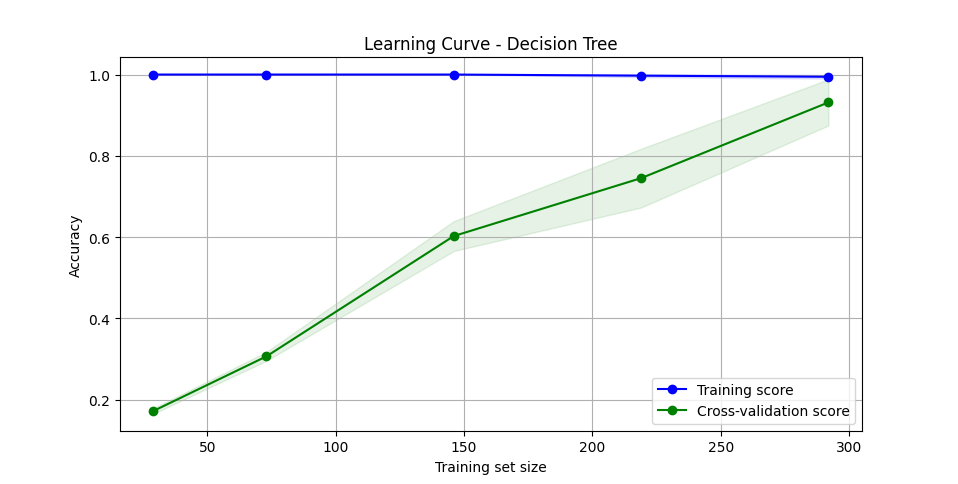
\includegraphics{images/plots/learning_2.png}} \\
        \hline
        \texttt{max\_depth=5, min\_samples\_split=5, ccp\_alpha=0.005, criterion=gini} &
        \adjustbox{max width=\linewidth,max height=3cm}{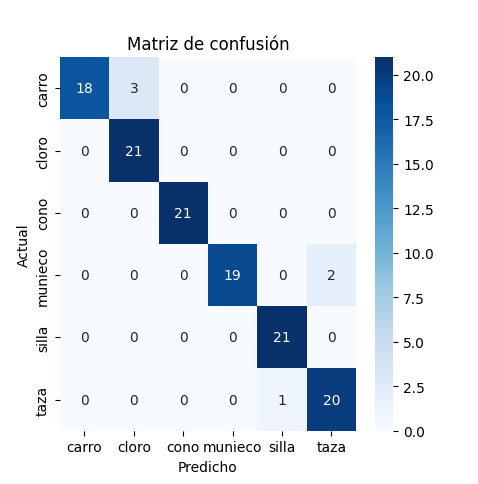
\includegraphics{images/plots/heap_3.png}} &
        \adjustbox{max width=\linewidth,max height=3cm}{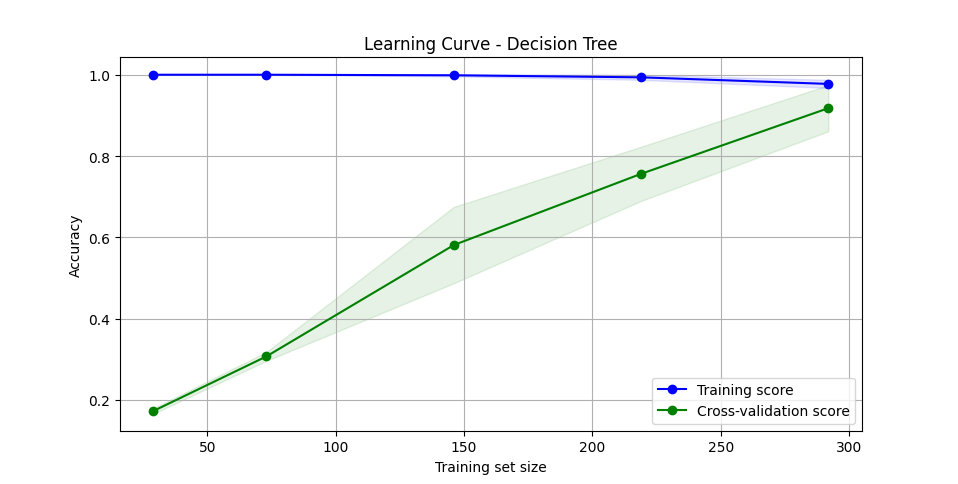
\includegraphics{images/plots/learning_3.png}} \\
        \hline
        \texttt{max\_depth=4, min\_samples\_split=5, ccp\_alpha=0.005, criterion=gini} &
        \adjustbox{max width=\linewidth,max height=3cm}{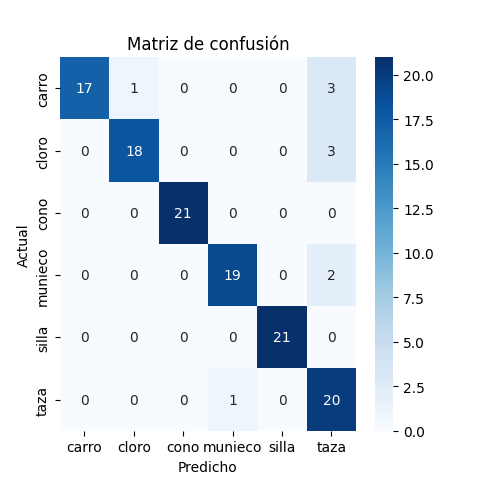
\includegraphics{images/plots/heap_4.png}} &
        \adjustbox{max width=\linewidth,max height=3cm}{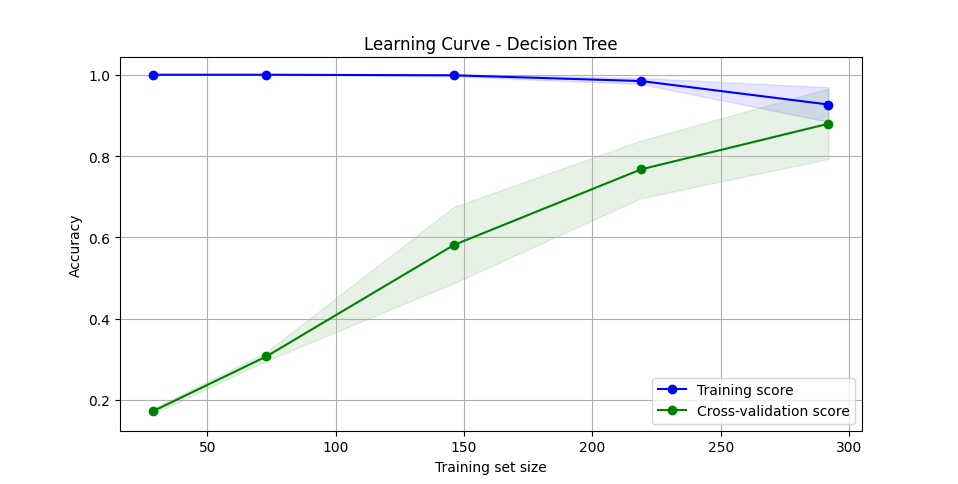
\includegraphics{images/plots/learning_4.png}} \\
        \hline
    \end{tabular}
\end{table}
\section{Conclusiones}
Tenemos dos conjuntos de datos, uno con 436 ejemplos y otro con 498 ejemplos, sin embargo, comparando entre ambos casos, tiene más estabilidad el modelo con el primer dataset que el segundo. En algunos casos, se llega a mejorar el accuracy de validación, pero realmente es poco. EL mejor modelo que se pudo observar, tanto por equilibrio entre accuracy y diferencia entre los valores es el primero y el tercero del primer conjunto de datos,(Tabla \ref{tab:comparacion_modelos_dt}).La poda de $0.005$ y $0.001$ no marca una diferencia entre el primero y el tercero.

Sin embargo, lo preocupante es que en un principio el entrenamiento infiera demasiado bien los datos, pero si existe al menos un contraste entre los valores de validación que con los de entrenamiento, y el incremento gradual permite observar que si está aprendiendo. Además, con el conjunto de datos extendido se puede demostrar que si está llegando a un punto de convergencia. 
Este modelo en primeras instancias se podría mejorar con limpiezas más finas de los datos,además, de cambiar la disposición entre un carro y la botella de cloro. Si esto no se puede, la otra cuestión podría ser someterlo a mayores pruebas, ya que, si bien, para generar la curva de aprendizaje, se necesita validación cruzada. También se podría someter a esa validación previa. Otra situación llegaría a ser en la reducción de dimensionalidad, se pueden calcular numéricamente las covarianzas entre las variables y eliminarlas o compactarlas
\bibliographystyle{IEEEtran}
\bibliography{referencias}

\end{document}
